\documentclass[supercite]{Experimental_Report}
\title{计算机系统基础实验报告}
\author{阮云轩}
%\coauthor{张三、李四}
\school{}
\classnum{智科2402}
\stunum{U202490035}
%\costunum{U202115631、U202115631}
\instructor{赵进} % 该系列实验报告模板由华科大计院教师陈加忠制作
\date{2025年12月2日}

\usepackage{algorithm, multirow}
\usepackage{algpseudocode}
\usepackage{amsmath}
\usepackage{amsthm}
\usepackage{framed}
\usepackage{mathtools}
\usepackage{subcaption}
\usepackage{xltxtra} %提供了针对XeTeX的改进并且加入了XeTeX的LOGO, 自动调用xunicode宏包(提供Unicode字符宏)
\usepackage{bm}
\usepackage{tikz}
\usepackage{tikzscale}
\usepackage{pgfplots}
\usepackage{listings}
\usepackage{tocloft}
%\usepackage{enumerate}

\lstdefinestyle{commonCodeStyle}{
	language = C, % 假设主要是C语言代码，可按需更改语言类型
	basicstyle=\ttfamily\footnotesize, % 设置字体为等宽且小一号字体，方便排版
	breaklines = true, % 自动换行
	breakatwhitespace = true, % 尽量在空白处换行
	columns=flexible, % 灵活调整列宽，让代码适应页面宽度
	numbers=left, % 在代码左侧显示行号
	numberstyle=\tiny\color{gray}, % 行号的样式，设置为小字号灰色字体
	keywordstyle=\color{blue}\bfseries, % 关键字样式，加粗蓝色显示
	commentstyle=\itshape, % 注释样式，斜体绿色显示
	stringstyle=\color{magenta}, % 字符串样式，紫红色显示
	showstringspaces=false % 取消显示字符串中的空格，放在正确位置
}

\lstdefinestyle{mycode}{
	language = C,
	basicstyle=\ttfamily,
	breaklines = true,
	breakatwhitespace = true,
	stringstyle=\ttfamily, % 设置字符串的字体风格保持和基本字体一致（等宽字体），这里也可以根据喜好设置其他样式，若不想设置额外样式可不写此行
	showstringspaces=false % 关键在于这一行，用于取消显示字符串中的空格
}
%\usepackage{enumerate}

\pgfplotsset{compat=1.16}

\newcommand{\cfig}[3]{
	\begin{figure}[htb]
		\centering
		\includegraphics[width=#2\textwidth]{images/#1.tikz}
		\caption{#3}
		\label{fig:#1}
	\end{figure}
}

\newcommand{\sfig}[3]{
	\begin{subfigure}[b]{#2\textwidth}
		\includegraphics[width=\textwidth]{images/#1.tikz}
		\caption{#3}
		\label{fig:#1}
	\end{subfigure}
}

\newcommand{\xfig}[3]{
	\begin{figure}[htb]
		\centering
		#3
		\caption{#2}
		\label{fig:#1}
	\end{figure}
}
\renewcommand{\cftlstlistingpresnum}{代码 }
\renewcommand{\cftlstlistingaftersnum}{:}
\setlength{\cftlstlistingnumwidth}{3.5em}

\newcommand{\rfig}[1]{\autoref{fig:#1}}
\newcommand{\ralg}[1]{\autoref{alg:#1}}
\newcommand{\rthm}[1]{\autoref{thm:#1}}
\newcommand{\rlem}[1]{\autoref{lem:#1}}
\newcommand{\reqn}[1]{\autoref{eqn:#1}}
\newcommand{\rtbl}[1]{\autoref{tbl:#1}}

\algnewcommand\Null{\textsc{null }}
\algnewcommand\algorithmicinput{\textbf{Input:}}
\algnewcommand\Input{\item[\algorithmicinput]}
\algnewcommand\algorithmicoutput{\textbf{Output:}}
\algnewcommand\Output{\item[\algorithmicoutput]}
\algnewcommand\algorithmicbreak{\textbf{break}}
\algnewcommand\Break{\algorithmicbreak}
\algnewcommand\algorithmiccontinue{\textbf{continue}}
\algnewcommand\Continue{\algorithmiccontinue}
\algnewcommand{\LeftCom}[1]{\State $\triangleright$ #1}

\newtheorem{thm}{定理}[section]
\newtheorem{lem}{引理}[section]

\makeatletter
% 定义 \subsubsubsection 命令
\newcommand{\subsubsubsection}{\@startsection{subsubsubsection}{4}{\z@}{-3.25ex plus -1ex minus -.2ex}{1.5ex plus.2ex}{\normalfont\Large\bfseries}}
% 定义 \subsubsubsubsection 命令
\newcommand{\subsubsubsubsection}{\@startsection{subsubsubsubsection}{5}{\z@}{-3.25ex plus -1ex minus -.2ex}{1.5ex plus.2ex}{\normalfont\large\bfseries}}
% 定义 \subsubsubsubsubsection 命令
\newcommand{\subsubsubsubsubsection}{\@startsection{subsubsubsubsubsection}{6}{\z@}{-3.25ex plus -1ex minus -.2ex}{1.5ex plus.2ex}{\normalfont\normalsize\bfseries}}
\makeatother

\colorlet{shadecolor}{black!15}

\theoremstyle{definition}
\newtheorem{alg}{算法}[section]

\def\thmautorefname~#1\null{定理~#1~\null}
\def\lemautorefname~#1\null{引理~#1~\null}
\def\algautorefname~#1\null{算法~#1~\null}

\begin{document}
	
	\maketitle
	
	\clearpage
	
	\pagenumbering{Roman}
	
	\tableofcontents[level=2]
	
	\clearpage
	
	\pagenumbering{arabic}
	
	\listoflistings
	
	\section{引言}
	本实验旨在深入探究计算器系统的底层运作机制，从高级语言的抽象层下沉至内存与位操作的具体实现层。在现代计算器科学中，理解数据在内存中的物理布局以及 CPU 处理数据的逻辑门电路原理，是编写高效、健壮代码的基石。
	
	通过实验任务，我们将直观地观测计算器内存的各种现象，模拟 CPU 的 ALU（算术逻辑单元）行为，这不仅是对逻辑思维的锻炼，更是对计算器二进制本质的探究。通过 GDB 调试工具的动态追踪，我们得以「打开黑盒」，亲眼见证数据在寄存器与内存间流转的微观过程。
	
	
	\section{数据表示和等效运算}
	\subsection{实验目的与要求}
	(1) 熟练掌握程序开发的基本方法，包括程序的编译、链接和调试；
	
	(2) 熟悉数据的表示形式；
	
	(3) 熟悉地址的计算方法、地址的内存转换；
	
	(4) 用常见的按位操作（移位、按位与/或/非/异或）等实现运算表达式的等效运算。
	
	\subsection{实验内容}
	\subsubsection*{任务1 数据压缩}
	
	定义了结构 \texttt{student}，以及结构数组变量 \texttt{old\_s[N]}, \texttt{new\_s[N]}; ($N=5$)
	
	% --- 修改部分：不再使用 lstlisting，改用普通文本加换行 ---
	\noindent \texttt{struct student \{} \\
	\texttt{\hspace*{2em} char  name[8];} \\
	\texttt{\hspace*{2em} short  age;} \\
	\texttt{\hspace*{2em} float  score;} \\
	\texttt{\hspace*{2em} char  remark[200];  // 备注信息} \\
	\texttt{\};}
	% ----------------------------------------------------
	
	编写程序，将 \texttt{old\_s[N]} 中的所有信息依次紧凑(压缩)存放到一个字符数组 \texttt{message} 中，然后从 \texttt{message} 解压缩到结构数组 \texttt{new\_s[N]} 中。打印压缩前(\texttt{old\_s})、解压后(\texttt{new\_s})的结果，以及压缩前、压缩后存放数据的长度。
	
	\paragraph{要求：}
	
	\begin{enumerate}
		\item 输入的第0个人姓名(name)为自己的名字，分数为学号的最后两位；
		
		\item 编写指定接口的函数完成数据压缩。压缩函数有两个：
		
		% --- 修改部分：直接用 textt 显示函数声明，手动转义下划线 ---
		\noindent \texttt{int  pack\_student\_bytebybyte(student* s, int sno, char *buf);} \\
		\texttt{int  pack\_student\_whole(student* s, int sno, char *buf);}
		% --------------------------------------------------------
		
		$s$ 为待压缩数组的起始地址；$sno$ 为压缩人数；$buf$ 为压缩存储区的首地址；两个函数的返回均是调用函数压缩后的字节数。\texttt{pack\_student\_bytebybyte} 要求一个字节一个字节的向 $buf$ 中写数据；\texttt{pack\_student\_whole} 要求对 \texttt{short}、\texttt{float} 字段都只能用一条语句整体写入，用 \texttt{strcpy} 实现串的写入。
		
		\item 使用指定方式调用压缩函数：
		\texttt{old\_s} 数组的前 $N1$（$N1=2$）个记录压缩调用 \texttt{pack\_student\_bytebybyte} 完成；后 $N2$（$N2=3$）个记录压缩调用 \texttt{pack\_student\_whole}，两种压缩函数都只调用1次。
		
		\item 使用指定的函数完成数据的解压。解压函数的格式：
		
		% --- 修改部分 ---
		\noindent \texttt{int restore\_student(char *buf, int len, student* s);}
		% ---------------
		
		$buf$ 为压缩区域存储区的首地址；$len$ 为 $buf$ 中存放数据的长度；$s$ 为存放解压数据的结构数组的起始地址；返回解压的人数。解压时不允许使用函数接口之外的信息（即不允许定义其他全局变量）。
		
		\item 仿照调试时看到的内存数据，以十六进制的形式，输出 \texttt{message} 的前40个字节的内容，并与调试时在内存窗口观察到的 \texttt{message} 的前40个字节比较是否一致。
		
		\item 对于第0个学生的 \texttt{score}，根据浮点数的编码规则指出其各部分的编码，并与观察到的内存表示比较，验证是否一致。
		
		\item 指出结构数组中各元素的存放规律，指出字符串数组、\texttt{short} 类型的数、\texttt{float} 型的数的存放规律。
	\end{enumerate}
	
	\subsubsection*{任务2 编写位运算程序}
	按照要求完成给定的功能，并自动判断程序的运行结果是否正确。（从逻辑电路与门、或门、非门等等角度，实现CPU的常见功能。所谓自动判断，即用简单的方式实现指定功能，并判断两个函数的输出是否相同。）
	
	\begin{enumerate}
		\item \texttt{int absVal(int x);} 返回 x 的绝对值 \\
		仅使用 \verb|!|、 \verb|~|、 \verb|&|、 \verb|^|、 \verb|||、 \verb|+|、 \verb|<<|、 \verb|>>|， 运算次数不超过 10次。\\
		判断函数： \texttt{int absVal\_standard(int x) \{ return (x < 0) ? -x : x;\}}
		
		\item \texttt{int negate(int x);} 不使用负号，实现 $-x$ \\
		判断函数： \texttt{int netgate\_standard(int x) \{ return -x;\}}
		
		\item \texttt{int bitAnd(int x, int y);} 仅使用 \verb|~| 和 \verb|||，实现 \verb|&| \\
		判断函数： \texttt{int bitAnd\_standard(int x, int y) \{ return x \& y;\}}
		
		\item \texttt{int bitOr(int x, int y);} 仅使用 \verb|~| 和 \verb|&|，实现 \verb|||
		
		\item \texttt{int bitXor(int x, int y);} 仅使用 \verb|~| 和 \verb|&|，实现 \verb|^|
		
		\item \texttt{int isTmax(int x);} 判断x是否为最大的正整数（7FFFFFFF），\\
		只能使用 \verb|!|、 \verb|~|、 \verb|&|、 \verb|^|、 \verb|||、 \verb|+|
		
		\item \texttt{int bitCount(int x);} 统计x的二进制表示中 1 的个数 \\
		只能使用 \verb|!| \verb|~| \verb|&| \verb|^| \verb||| \verb|+| \verb|<<| \verb|>>|，运算次数不超过 40次
		
		\item \texttt{int bitMask(int highbit, int lowbit);} 产生从 lowbit 到 highbit 全为1，其他位为0的数。例如 \texttt{bitMask(5,3) = 0x38}；要求只使用 \verb|!| \verb|~| \verb|&| \verb|^| \verb||| \verb|+| \verb|<<| \verb|>>|；运算次数不超过 16次。
		
		\item \texttt{int addOK(int x, int y);} 当 $x+y$ 会产生溢出时返回1，否则返回 0 \\
		仅使用 \verb|!|、 \verb|~|、 \verb|&|、 \verb|^|、 \verb|||、 \verb|+|、 \verb|<<|、 \verb|>>|， 运算次数不超过 20次
		
		\item \texttt{int byteSwap(int x, int n, int m);} 将x的第n个字节与第m个字节交换，返回交换后的结果。 n、m的取值在 0\textasciitilde 3之间。\\
		例：\texttt{byteSwap(0x12345678, 1, 3) = 0x56341278} \\
		\texttt{byteSwap(0xDEADBEEF, 0, 2) = 0xDEEFBEAD} \\
		仅使用 \verb|!|、 \verb|~|、 \verb|&|、 \verb|^|、 \verb|||、 \verb|+|、 \verb|<<|、 \verb|>>|， 运算次数不超过 25次
		
		\item \texttt{int bang(int x);} 当 $x=0$ 时，返回 1; 其他情况返回 0。实现逻辑非(\verb|!|) \\
		例：\texttt{bang(3) = 0;} \texttt{bang(0) = 1;} \\
		仅使用 \verb|~|、 \verb|&|、 \verb|^|、 \verb||| 、\verb|+|、 \verb|<<|、 \verb|>>|，运算次数不超过 12次 \\
		提示：只有当 $x=0$ 时，$x$ 与 $-x$ 的最高二进制位会同时为0。
		
		\item \texttt{int bitParity(int x);} 当 $x$ 有奇数个二进制位0，返回1；否则返回0 \\
		例：\texttt{bitParity(5) = 0;} \texttt{bitParity(7) = 1;} \\
		仅使用 \verb|!| 、\verb|~|、 \verb|&|、 \verb|^|、 \verb||| 、\verb|+| 、\verb|<<| 、\verb|>>|，运算次数不超过 20次。\\
		提示：只有当 $x$ 的高字与低字的对应位（第0位对应第16位，第1位对应第17位，依次类推）同时为1，则出现了成对的二进制位1，此时，可以将对应的二进制位置为0，不会影响二进制位1的个数的奇偶性判断。
	\end{enumerate}
	\subsection{实验记录及问题回答}
	\subsubsection{任务1  数据存放的压缩与解压编程}
	\subsubsubsection{分析}
	首先分析待压缩的数据结构，student 结构体中的姓名 (name) 和备注 (remark) 分别固定占用 8 和 200 个字节，但实际输入的姓名或备注往往很短，这导致内存中存在大量用于占位的无效 0x00 字节，这就是主要的压缩空间；其次是年龄 (age)，虽然 short 类型占 2 字节，但人的年龄通常不超过 255，高位字节几乎恒为 0，也可以省去；只有分数 (score) 因遵循 IEEE 754 浮点数标准，结构复杂且无冗余，无法简单压缩。在 GDB 调试中观察内存发现，输入的中文姓名呈现 UTF-8 编码（如 e5 bd ad...），且年龄 18 在内存中显示为 12 00，验证了 x86 架构的小端序存储模式。压缩前，这些有效数据被大片的 0 隔开，呈现稀疏状态；压缩后，通过指针操作去除了所有填充的 0，名字后紧接分隔符和年龄的低位字节，数据变得非常紧凑，证明了压缩算法有效消除了空间浪费。
	
	测试范例
	
	阮云轩 18 35 goodgoodstudydaydayup
	
	Kit 197 70.5 Smart
	
	Kingsley 3 21.5 Macao
	
	Ryan 14 66.6 Rich
	
	Kevin 20 2.33 Hust
	
	然后我们输入数据后看下内存空间(\ref{fig1-1})，可以观察到，我们的空间利用率是十分低效的，有很多空内存的位置，于是我们需要想办法去设计算法去压缩我们的内存空间，提高利用率。
	\begin{figure}[H]
		\begin{center}
			
\includegraphics[scale=0.7]{images/1-1.jpg}
			\caption{压缩前内存}
			\label{fig1-1}
		\end{center}
	\end{figure}
	
	\subsubsubsection{算法设计}
	pack student bytebybyte
	
	该函数采用了「动态缓冲」的策略来处理未知的压缩长度。算法利用 C++ 的 std::vector<char> 作为临时容器，通过指针 char* p 强制转换结构体地址，对内存进行字节级别的遍历。在处理字符串字段时，程序会检测非零字符并将其压入容器，遇到空字符或达到长度上限时停止，并手动追加一个 0 作为分隔符；在处理数值时，指针会跳过 age 的高位字节仅读取低位，并连续读取 score 的 4 个字节。最终，程序根据 vector 的总大小动态分配输出缓冲区，并使用 memcpy 完成数据的导出，这种方式有效避免了手动管理内存边界的复杂性。
	
	\begin{figure}[H]
		\begin{center}
			
\includegraphics[scale=0.3]{images/1-2.jpg}
			\caption{pack student bytebybyte}
			\label{fig1-2}
		\end{center}
	\end{figure}
	
	pack student whole
	
	该函数采用了「两遍扫描（Two-pass）」的策略，旨在优化内存分配效率并利用块操作提高写入速度。第一遍扫描专注于计算空间，通过遍历所有学生记录，利用 strlen 获取姓名和备注的实际长度（并计入分隔符开销），加上年龄（1字节）和分数（4字节）的固定开销，累加得出精确的缓冲区总大小。第二遍扫描则执行实际的写入操作，利用一个光标指针 p 在已分配的内存中移动，使用 strcpy 快速写入字符串，使用 memcpy 直接拷贝数值数据。每写入一个字段，游标便向后偏移相应的字节数，实现了数据在内存中的紧凑排列。
	
	\begin{figure}[H]
		\begin{center}
			
\includegraphics[scale=0.3]{images/1-3.jpg}
			\caption{pack student whole}
			\label{fig1-3}
		\end{center}
	\end{figure}
	
	restore student
	
	解压函数执行的是压缩的逆过程，核心逻辑是通过维护一个读取指针来解析紧凑的字节流。在还原字符串时，算法循环读取字节直到遇到分隔符 \0，将字符逐一复制回目标结构体的数组中，并关键性地使用 memset 将数组剩余的空间清零，防止内存脏数据残留。在还原数值时，程序读取 1 个字节赋值给 age 的低位，并强制将 age 的高位设为 0 以恢复 short 类型；随后连续读取 4 个字节，通过内存拷贝无损还原 float 类型的分数数据。整个过程循环进行，直到读取指针超出缓冲区边界。
	
	\begin{figure}[H]
		\begin{center}
			
\includegraphics[scale=0.3]{images/1-4.jpg}
			\caption{restore student}
			\label{fig1-4}
		\end{center}
	\end{figure}
	
	\subsubsubsection{运行结果}
	我们针对我们的测试范例，看看压缩后的内存空间是怎样的
	\begin{figure}[H]
		\begin{center}
			
\includegraphics[scale=0.7]{images/1-5.jpg}
			\caption{压缩后的内存空间}
			\label{fig1-5}
		\end{center}
	\end{figure}
	现在我们来解读一下压缩后的空间，我们以第一组学生数据为例去分析。
	
	首先我们的学生姓名是 "阮云轩"，因为我们使用的是 UTF-8 编码，每个汉字占用 3 个字节，对应数据段 0xe9 0x98 0xae (阮) 0xe9 0x9b 0xb2 (云) 0xe8 0xbb 0x92 (轩)，然后 0x00 表示数据段终止。
	
	然后年龄 18 对应 0x12 (十六进制)。
	
	分数 35 因为是 float 型存取（且为小端序存储），因此它对应 0x00 0x00 0x0c 0x42 (对应 IEEE 754 的 35.0)。
	
	最后是我们的备注 "goodgoodstudydaydayup"，它是 ASCII 码，比如 "good" 就对应 0x67 0x6f 0x6f 0x64，"study" 对应 0x73 0x74 0x75 0x64 0x79，"day" 对应 0x64 0x61 0x79，"up" 对应 0x75 0x70，如此类推，直到最后一个 0x00 结束符，这就完成了我们一个学生的数据压缩。
	
	\subsubsection{任务2  编写位运算程序}
	\subsubsubsection{算法设计}
	1.absVal (绝对值运算) 
	
	该算法的核心在于利用算术右移构造掩码来处理符号。通过将 x 右移 31 位，当 x 为正数时得到全 0 的掩码，当 x 为负数时得到全 1 的掩码（即 -1）；利用异或运算的特性，任何数与 0 异或保持不变，与 -1 异或相当于按位取反，最后再加上掩码的最低位（0 或 1），从而完美实现了「正数不变，负数取反加一」的绝对值逻辑。
	
	2.negate (取负运算) 
	
	这个函数直接利用了计算器二进制补码（Two's Complement）的定义来实现。在计算器系统中，一个整数的相反数定义为该数按位取反（~x）之后再加 1，这是一个最基础的底层运算规则，因此无需任何额外的条件判断即可直接算出 -x。
	
	3.bitAnd (按位与运算) 
	
	该算法应用了集合论中的德摩根定律（De Morgan's Laws）来绕过限制。德摩根定律指出「非（A 与 B）」等价于「（非 A）或（非 B）」，因此算法先对 x 和 y 分别进行按位取反，然后对它们进行按位或运算，最后再对整个结果取反，从而在不直接使用 & 运算符的情况下等效实现了按位与的功能。
	
	4.bitOr (按位或运算) 
	
	与按位与函数类似，这里同样运用了德摩根定律的变换形式。根据定律，「A 或 B」等价于「非（（非 A）与（非 B））」，算法通过先将两个输入数 x 和 y 分别取反，接着进行按位与运算，最后再对结果取反，成功地仅用 ~ 和 \& 两个运算符模拟出了按位或的逻辑。
	
	5.bitXor (按位异或运算) 
	
	异或的定义是「两个位不同则为 1」，这可以拆解为两种情况：「x 为 0 且 y 为 1」或者「x 为 1 且 y 为 0」。算法通过组合使用取反和按位与运算符，分别构造出这两部分的逻辑表达式（即 ~x \& y 和 x \& ~y），然后再利用德摩根定律将它们合并（模拟或运算），从而实现了异或功能。
	
	6.isTmax (判断最大正整数) 
	
	判断一个数是否为最大正整数（0x7FFFFFFF），最直接的方法是利用异或运算「相同为 0」的特性。算法将输入 x 与标准的最大正整数 0x7FFFFFFF 进行异或，如果两者相等，异或结果必为 0，最后对这个结果进行逻辑非（!）运算，即可返回 1 表示真，否则返回 0。
	
	7.bitCount (统计 1 的个数) 
	
	该算法采用了高效的分治策略（并行计数法）。它不逐位遍历，而是通过一系列特定的掩码（如 0x5555...、0x3333...），先计算每两个相邻位中 1 的个数，再计算每四位中 1 的个数，以此类推，层层累加合并，最终在极少的步骤内计算出 32 位整数中所有 1 的总和。
	
	8.bitMask (生成掩码) 
	
	生成从 lowbit 到 highbit 全为 1 的掩码，思路是构造两个边界。算法首先构造一个从第 0 位到 highbit 位全为 1 的数，再利用取反和移位构造出一个屏蔽掉 lowbit 以下位置的掩码，通过这两部分的位运算组合（或减法逻辑的变体），精确地保留了指定区间内的 1，其余位置均为 0。
	
	9.addOK (加法溢出判断) 
	
	检测加法溢出的关键在于符号位的异常变化。溢出只可能发生在两个同号数相加的情况下，即「正加正得负」或「负加负得正」。算法通过移位提取出两个操作数以及结果的符号位，利用异或门判断操作数是否同号以及结果是否变号，当满足溢出条件时返回 1，否则返回 0。
	
	10.byteSwap (字节交换) 
	
	算法的核心是「提取、清零、回填」。首先通过位移和与运算分别提取出第 n 个和第 m 个字节的数值，同时构造掩码将原数中这两个字节的位置清零；接着将提取出的两个字节数值移动到对方的目标位置，最后与清零后的原数进行按位或合并，完成了特定字节的交换。
	
	11.bang (逻辑非运算) 
	
	实现逻辑非的难点在于区分 0 和非 0，算法利用了二补码的一个特殊性质：只有 0 的相反数（-0）符号位与原数相同（都是 0），而任何非 0 数的原数或其相反数中必有一个符号位为 1。通过将 x 与 -x 进行按位或并右移取出符号位，再加 1，即可将 0 映像为 1，将非 0 数映射为 0。
	
	12.bitParity (奇偶校验) 
	该算法利用了异或运算的「折迭」特性来消除成对的 1。算法不断将数据的高一半位与低一半位进行异或（如高 16 位与低 16 位异或，结果存入低 16 位），这样相同的位会抵消为 0，经过多次折迭后，最低位保留的值就代表了原始数据中 1 的个数是奇数还是偶数。
	
	然后我们对比一下我们的输出对比下结果，可以看到是一致的，说明我们的算法设计是对的
	\begin{figure}[H]
		\begin{center}
			
\includegraphics[scale=0.6]{images/1-6.jpg}
			\caption{对比}
			\label{fig1-6}
		\end{center}
	\end{figure}
	
	\subsection{体会}
	本次实验是探索计算器底层机制的第一步，通过对数据存储与运算的具体实践，我获得了以下的体会：
	
	1. 从内存视角审视数据结构
	
	在数据压缩任务中，我打破了以往对结构体（Struct）的抽象认知。通过分析内存布局，我直观地看到了编译程序为满足内存对齐而插入的填充字节，以及定长数组带来的空间冗余。通过指针操作将数据「串行化」为紧凑字节流的过程，不仅验证了 x86 架构的**小端序（Little Endian）**特性，更让我掌握了在字节层面精确控制数据存储的方法，理解了「空间优化」在底层编程中的实现代价。
	
	2. 仿真硬件层的运算逻辑
	
	位运算任务迫使我脱离高级语言的语法糖，转而使用**算术逻辑单元（ALU）的思维方式解决问题。在受限的运算符下，我深刻体会到了二补码（Two's Complement）设计的精妙——它让加减法在硬件电路中得以统一。同时，通过构造掩码（Mask）**和逻辑门组合来实现条件判断与算术运算，锻炼了我对二进制位的微观操控能力。
	
	\section{汇编和C的混合编程及优化}
	\subsection{实验目的与要求}
	(1) 熟练掌握程序开发平台(VS2019/VS2022/VS2023) 下C和汇编语言的混合编程方法；
	
	(2) 熟悉掌握常用机器指令的使用方法；
	
	(3) 掌握代码优化的基本方法，提高程序运行速度
	
	\subsection{实验内容}
	\subsubsection{任务1 用C语言编写一个学生成绩管理程序，具有平均成绩计算、按平均成绩从高到低排序、显示学生成绩的功能}
	定义了 结构 student，设有 N 个学生 
	
	struct student {
		
		char  name[8];
		
		char  sid[11];   //  如U202490035
		
		short  scores[8]; //  8门课的分数
		
		short  average;  //  平均分
		
	};
	
	要求：
	
	（1）	第0个人姓名(name)为自己的名字，sid为自己的学号； 
	
	（2）	对于函数“计算平均成绩”、“按平均成绩从高到低排序”分别计时，显示两个函数的时间开销；
	
	（3）	显示排序前、排序后的学生信息（姓名、学号、8门课的分数、平均分），一个学生一行。
	
	（4）	对“计算平均成绩”、“按平均成绩排序”函数的Debug版、Release版的运行效率进行对比，比较两个版本下的反汇编代码的差异，分析程序执行速度提高的原因。 
	
	\subsubsection{任务2  用汇编语言编写函数“计算平均成绩”，代替原来用C语言编写的函数}
	\subsubsection{任务3  对用汇编语言编写的“计算平均成绩”函数进行优化}
	\subsubsection{任务4  对排序函数进行算法优化}
	
	\subsection{算法设计}
	\subsubsection{任务1 用C语言编写一个学生成绩管理程序，具有平均成绩计算、按平均成绩从高到低排序、显示学生成绩的功能}
	我们设计了如下的计算平均值的函数，然后我们对比一下Debug版和Release版的区别
	\begin{lstlisting}[style=commonCodeStyle, caption={CalcAvg.cpp}, label={lst:2-1}]
		void CalcAvg_C(Student* s, int count) {
			for (int i = 0; i < count; ++i) {
				int sum = 0;
				for (int k = 0; k < 8; ++k) {
					sum += s[i].scores[k];
				}
				s[i].average = (short)(sum >> 3);
			}
		}
	\end{lstlisting}
	\begin{figure}[H],
		\begin{center}
			
\includegraphics[scale=0.6]{images/2-1.jpg}
			\caption{CalAvg}
			\label{fig2-1}
		\end{center}
	\end{figure}
	
	Debug版
	\begin{lstlisting}[style=commonCodeStyle, caption={debug.asm}, label={lst:2-2}]
		void CalcAvg_C(Student* s, int count) {
			004A4BF0  push        ebp  
			004A4BF1  mov         ebp,esp  
			004A4BF3  sub         esp,0E4h  
			004A4BF9  push        ebx  
			004A4BFA  push        esi  
			004A4BFB  push        edi  
			004A4BFC  lea         edi,[ebp-24h]  
			004A4BFF  mov         ecx,9  
			004A4C04  mov         eax,0CCCCCCCCh  
			004A4C09  rep stos    dword ptr es:[edi]  
			004A4C0B  mov         ecx,offset _AC749FA3_task1@cpp (04B4071h)  
			004A4C10  call        @__CheckForDebuggerJustMyCode@4 (04A1618h)  
			004A4C15  nop  
			for (int i = 0; i < count; ++i) {
				004A4C16  mov         dword ptr [ebp-8],0  
				004A4C1D  jmp         __$EncStackInitStart+2Ch (04A4C28h)  
				004A4C1F  mov         eax,dword ptr [ebp-8]  
				004A4C22  add         eax,1  
				004A4C25  mov         dword ptr [ebp-8],eax  
				004A4C28  mov         eax,dword ptr [ebp-8]  
				004A4C2B  cmp         eax,dword ptr [count]  
				004A4C2E  jge         __$EncStackInitStart+7Eh (04A4C7Ah)  
				int sum = 0;
				004A4C30  mov         dword ptr [ebp-14h],0  
				for (int k = 0; k < 8; ++k) {
					004A4C37  mov         dword ptr [ebp-20h],0  
					004A4C3E  jmp         __$EncStackInitStart+4Dh (04A4C49h)  
					004A4C40  mov         eax,dword ptr [ebp-20h]  
					004A4C43  add         eax,1  
					004A4C46  mov         dword ptr [ebp-20h],eax  
					004A4C49  cmp         dword ptr [ebp-20h],8  
					004A4C4D  jge         __$EncStackInitStart+6Ah (04A4C66h)  
					sum += s[i].scores[k];
					004A4C4F  imul        eax,dword ptr [ebp-8],29h  
					004A4C53  add         eax,dword ptr [s]  
					004A4C56  mov         ecx,dword ptr [ebp-20h]  
					004A4C59  movsx       edx,word ptr [eax+ecx*2+17h]  
					004A4C5E  add         edx,dword ptr [ebp-14h]  
					004A4C61  mov         dword ptr [ebp-14h],edx  
				}
				004A4C64  jmp         __$EncStackInitStart+44h (04A4C40h)  
				
				s[i].average = (short)(sum >> 3);
				004A4C66  mov         eax,dword ptr [ebp-14h]  
				004A4C69  sar         eax,3  
				004A4C6C  imul        ecx,dword ptr [ebp-8],29h  
				004A4C70  mov         edx,dword ptr [s]  
				004A4C73  mov         word ptr [edx+ecx+27h],ax  
			}
			004A4C78  jmp         __$EncStackInitStart+23h (04A4C1Fh)  
			
		}
		004A4C7A  pop         edi  
		004A4C7B  pop         esi  
		004A4C7C  pop         ebx  
		004A4C7D  add         esp,0E4h  
		004A4C83  cmp         ebp,esp  
		004A4C85  call        __RTC_CheckEsp (04A144Ch)  
		004A4C8A  mov         esp,ebp  
		004A4C8C  pop         ebp  
		004A4C8D  ret  
	\end{lstlisting}
	
	Release版
	\begin{lstlisting}[style=commonCodeStyle, caption={release.asm}, label={lst:2-3}]
		CalcAvg_C(students.data(), N);
		00FC1670  movsx       eax,word ptr [edx-0Ah]  
		00FC1674  lea         edx,[edx+29h]  
		00FC1677  movsx       ecx,word ptr [edx-35h]  
		00FC167B  add         ecx,eax  
		00FC167D  movsx       eax,word ptr [edx-31h]  
		00FC1681  add         ecx,eax  
		00FC1683  movsx       eax,word ptr [edx-2Fh]  
		00FC1687  add         ecx,eax  
		00FC1689  movsx       eax,word ptr [edx-2Dh]  
		00FC168D  add         ecx,eax  
		00FC168F  movsx       eax,word ptr [edx-2Bh]  
		00FC1693  add         ecx,eax  
		00FC1695  movsx       eax,word ptr [edx-27h]  
		00FC1699  add         ecx,eax  
		00FC169B  movsx       eax,word ptr [edx-29h]  
		00FC169F  add         ecx,eax  
		00FC16A1  sar         ecx,3  
		00FC16A4  mov         word ptr [edx-25h],cx  
		00FC16A8  sub         esi,1  
		00FC16AB  jne         main+1C0h (0FC1670h)  
	\end{lstlisting}
	
	我们设计了如下的计算平均值的函数，然后我们对比一下Debug版和Release版的区别
	我们再对比一下Sort函数的Debug版和Release版的区别，这是我们设计的Sort的源代码
	\begin{lstlisting}[style=commonCodeStyle, caption={sort.cpp}, label={lst:2-4}]
		void Sort_C(Student* s, int count) {
			for (int i = 0; i < count - 1; ++i) {
				bool swapped = false;
				for (int j = 0; j < count - 1 - i; ++j) {
					if (s[j].average < s[j + 1].average) { // 降序排序
						Student temp = s[j];
						s[j] = s[j + 1];
						s[j + 1] = temp;
						swapped = true;
					}
				}
				if (!swapped) break; 
			}
			
		} 
	\end{lstlisting}
	Debug版
	\begin{lstlisting}[style=commonCodeStyle, caption={debug.asm}, label={lst:2-5}]
		void CalcAvg_C(Student* s, int count) {
			004A4BF0  push        ebp  
			004A4BF1  mov         ebp,esp  
			004A4BF3  sub         esp,0E4h  
			004A4BF9  push        ebx  
			004A4BFA  push        esi  
			004A4BFB  push        edi  
			004A4BFC  lea         edi,[ebp-24h]  
			004A4BFF  mov         ecx,9  
			004A4C04  mov         eax,0CCCCCCCCh  
			004A4C09  rep stos    dword ptr es:[edi]  
			004A4C0B  mov         ecx,offset _AC749FA3_task1@cpp (04B4071h)  
			004A4C10  call        @__CheckForDebuggerJustMyCode@4 (04A1618h)  
			004A4C15  nop  
			for (int i = 0; i < count; ++i) {
				004A4C16  mov         dword ptr [ebp-8],0  
				004A4C1D  jmp         __$EncStackInitStart+2Ch (04A4C28h)  
				004A4C1F  mov         eax,dword ptr [ebp-8]  
				004A4C22  add         eax,1  
				004A4C25  mov         dword ptr [ebp-8],eax  
				004A4C28  mov         eax,dword ptr [ebp-8]  
				004A4C2B  cmp         eax,dword ptr [count]  
				004A4C2E  jge         __$EncStackInitStart+7Eh (04A4C7Ah)  
				int sum = 0;
				004A4C30  mov         dword ptr [ebp-14h],0  
				for (int k = 0; k < 8; ++k) {
					004A4C37  mov         dword ptr [ebp-20h],0  
					004A4C3E  jmp         __$EncStackInitStart+4Dh (04A4C49h)  
					004A4C40  mov         eax,dword ptr [ebp-20h]  
					004A4C43  add         eax,1  
					004A4C46  mov         dword ptr [ebp-20h],eax  
					004A4C49  cmp         dword ptr [ebp-20h],8  
					004A4C4D  jge         __$EncStackInitStart+6Ah (04A4C66h)  
					sum += s[i].scores[k];
					004A4C4F  imul        eax,dword ptr [ebp-8],29h  
					004A4C53  add         eax,dword ptr [s]  
					004A4C56  mov         ecx,dword ptr [ebp-20h]  
					004A4C59  movsx       edx,word ptr [eax+ecx*2+17h]  
					004A4C5E  add         edx,dword ptr [ebp-14h]  
					004A4C61  mov         dword ptr [ebp-14h],edx  
				}
				004A4C64  jmp         __$EncStackInitStart+44h (04A4C40h)  
				
				s[i].average = (short)(sum >> 3);
				004A4C66  mov         eax,dword ptr [ebp-14h]  
				004A4C69  sar         eax,3  
				004A4C6C  imul        ecx,dword ptr [ebp-8],29h  
				004A4C70  mov         edx,dword ptr [s]  
				004A4C73  mov         word ptr [edx+ecx+27h],ax  
			}
			004A4C78  jmp         __$EncStackInitStart+23h (04A4C1Fh)  
			
		}
		004A4C7A  pop         edi  
		004A4C7B  pop         esi  
		004A4C7C  pop         ebx  
		004A4C7D  add         esp,0E4h  
		004A4C83  cmp         ebp,esp  
		004A4C85  call        __RTC_CheckEsp (04A144Ch)  
		004A4C8A  mov         esp,ebp  
		004A4C8C  pop         ebp  
		004A4C8D  ret  
	\end{lstlisting}
	Release版
	\begin{lstlisting}[style=commonCodeStyle, caption={Release.asm}, label={lst:2-6}]
		Sort_C(students.data(), N);
		00FC1786  mov         eax,dword ptr [students]  
		00FC1789  mov         dword ptr [start],ecx  
		00FC178C  mov         dword ptr [ebp-28h],eax  
		00FC178F  nop  
		00FC1790  xor         cl,cl  
		00FC1792  lea         edx,[eax+29h]  
		00FC1795  mov         esi,edi  
		00FC1797  nop         word ptr [eax+eax]  
		00FC17A0  mov         ax,word ptr [edx-2]  
		00FC17A4  cmp         ax,word ptr [edx+27h]  
		00FC17A8  jge         main+33Ah (0FC17EAh)  
		00FC17AA  movups      xmm0,xmmword ptr [edx]  
		00FC17AD  mov         cl,byte ptr [edx-1]  
		00FC17B0  movups      xmm1,xmmword ptr [edx-29h]  
		00FC17B4  mov         al,byte ptr [edx+28h]  
		00FC17B7  movups      xmm2,xmmword ptr [edx-19h]  
		00FC17BB  movq        xmm3,mmword ptr [edx-9]  
		00FC17C0  movups      xmmword ptr [edx-29h],xmm0  
		00FC17C4  movups      xmm0,xmmword ptr [edx+10h]  
		00FC17C8  movups      xmmword ptr [edx-19h],xmm0  
		00FC17CC  movq        xmm0,mmword ptr [edx+20h]  
		00FC17D1  movups      xmmword ptr [edx],xmm1  
		00FC17D4  movups      xmmword ptr [edx+10h],xmm2  
		00FC17D8  movq        mmword ptr [edx+20h],xmm3  
		00FC17DD  movq        mmword ptr [edx-9],xmm0  
		00FC17E2  mov         byte ptr [edx+28h],cl  
		00FC17E5  mov         cl,1  
		00FC17E7  mov         byte ptr [edx-1],al  
		00FC17EA  add         edx,29h  
		00FC17ED  sub         esi,1  
		00FC17F0  jne         main+2F0h (0FC17A0h)  
		00FC17F2  test        cl,cl  
		00FC17F4  je          main+34Eh (0FC17FEh)  
		00FC17F6  mov         eax,dword ptr [ebp-28h]  
		00FC17F9  dec         edi  
		00FC17FA  test        edi,edi  
		00FC17FC  jg          main+2E0h (0FC1790h)  
	\end{lstlisting}
	
	
	「通过对比反汇编代码（如图所示），Debug 版为了支持调试功能，未开启优化，导致产生了大量冗余的内存读写指令（如频繁访问 [ebp-xx]），严格遵循源代码逻辑。
	
	而 Release 版 开启了 O2 级优化，编译程序将变量尽量保留在 寄存器 (如 eax, ecx) 中以减少内存访问延迟；同时将除法运算 sum/8 优化为位运算 sar (右移)，并精简了循环结构。这解释了为什么 Release 版的运行时间（xx微秒）远低于 Debug 版。」
	
	我们可以观察到以下性质
	
	1. 指令数量与执行速度
	Debug 版：指令非常冗长。即使是一个简单的加法，也需要好几条 mov 指令把数据从内存搬到寄存器，算完再搬回内存。
	
	Release 版：指令极少。同样的功能可能只需要几行代码。指令少意味着 CPU 执行的周期更少，速度更快。
	
	2. 数据存储方式：堆栈 vs 寄存器
	
	Debug 版：严重依赖 堆栈 (Stack)。
	
	存在大量的 [ebp-8], [ebp-14h] 等操作。这是在频繁地读写内存（RAM/Cache）。
	
	目的：为了让在调试时，随时把鼠标移到变量上都能看到它的值。
	
	Release 版：充分利用 寄存器 (Register)。
	
	您会看到大量的 eax, ecx, edx 操作。数据直接在 CPU 内部流转，很少访问内存。
	
	优势：寄存器的速度比内存快几百倍。
	
	3. 内存寻址与计算优化
	Debug 版：笨拙地计算地址。比如要访问数组 s[i]，老老实实地做乘法、加法来算出地址。
	
	Release 版：直接计算偏移量。编译程序会预判数据的位置，省去了运行时的 add 和 imul (乘法) 指令。
	
	4. 循环与运算优化
	
	移位代替除法：
	
	Debug 版：可能会调用除法指令或保留除法逻辑。
	
	Release 版：直接变成了 sar ecx, 3 (右移 3 位)。因为在二进制中，右移 3 位就等于除以 8，但移位指令的速度比除法快得多。
	
	循环展开：
	
	Debug 版会老实地执行 jmp 跳转，一次次循环。
	
	Release 版可能会把循环「拆开」，一次处理多个数据，减少 CPU 跳转预测失败的风险。
	
	
	\subsubsection{任务2  用汇编语言编写函数“计算平均成绩”，代替原来用C语言编写的函数}
	汇编设计如下：
	\begin{lstlisting}[style=commonCodeStyle, caption={CalcAvg.asm}, label={lst:2-7}]
		.686P               ; 允许使用 Pentium Pro 指令集
		.model flat, C      ; 使用 C 语言调用约定 (参数从右往左入栈)
		
		; Name(8) + Sid(11) = 19
		OFFSET_SCORES equ 19
		; 19 + 8*2 = 35
		OFFSET_AVG    equ 35
		STRUCT_SIZE   equ 37
		
		.code
		CalcAvg_ASM PROC
		push ebp
		mov ebp, esp
		push ebx            ; 保存被调用者保存寄存器
		push esi
		push edi
		
		mov esi, [ebp + 8]  ; ESI = s (当前学生指针)
		mov ecx, [ebp + 12] ; ECX = count (循环计数器)
		
		; 如果人数 <= 0，直接退出
		test ecx, ecx
		jz _Exit
		
		_Loop_Student:
		push ecx 
		
		xor eax, eax        ; EAX = sum = 0
		lea ebx, [esi + OFFSET_SCORES] ; EBX 指向 scores 数组
		mov ecx, 8       
		
		_Loop_Score:
		movsx edx, word ptr [ebx]
		add eax, edx        
		add ebx, 2      
		dec ecx
		jnz _Loop_Score    
		
		; sum / 8 等同于 sum 右移 3 位
		sar eax, 3      
		
		; --- 存回结构体 ---
		mov word ptr [esi + OFFSET_AVG], ax
		
		; --- 移动到下一个学生 ---
		add esi, STRUCT_SIZE
		
		pop ecx      
		dec ecx
		jnz _Loop_Student 
		
		_Exit:
		pop edi
		pop esi
		pop ebx
		pop ebp
		ret
		CalcAvg_ASM ENDP
		
		END
	\end{lstlisting}
	\begin{figure}[H],
		\begin{center}
			
\includegraphics[scale=0.6]{images/2-2.jpg}
			\caption{CalAvg}
			\label{fig2-2}
		\end{center}
	\end{figure}
	注意运行时间，可以看到是十分快的，比原本的用C编写的要快
	
	
	\subsubsection{任务3  对用汇编语言编写的“计算平均成绩”函数进行优化}
	\begin{lstlisting}[style=commonCodeStyle, caption={CalcAvg.asm}, label={lst:2-8}]
		.686P
		.model flat, C
		
		; 定义偏移量 (与 C++ 对齐)
		OFFSET_SCORES equ 19
		OFFSET_AVG    equ 35
		STRUCT_SIZE   equ 37
		
		.code
		
		CalcAvg_ASM_Opt PROC uses esi,
		ptr_data:DWORD, ; [ebp+8]
		count:DWORD     ; [ebp+12]
		
		mov esi, ptr_data       ; ESI = 当前学生指针
		mov ecx, count          ; ECX = 学生总数
		
		test ecx, ecx
		jz _Exit
		
		_Loop_Student:
		; --- 优化核心：循环展开 ---
		; 不再使用 loop 指令，而是直接写 8 次加法
		; 这样消除了循环控制指令 (dec, jnz) 的开销，流水线更顺畅
		
		xor eax, eax       
		
		
		add ax, word ptr [esi + 19] ; 第1门课
		add ax, word ptr [esi + 21] ; 第2门课
		add ax, word ptr [esi + 23] ; 第3门课
		add ax, word ptr [esi + 25] ; 第4门课
		add ax, word ptr [esi + 27] ; 第5门课
		add ax, word ptr [esi + 29] ; 第6门课
		add ax, word ptr [esi + 31] ; 第7门课
		add ax, word ptr [esi + 33] ; 第8门课
		
		sar eax, 3 
		
		mov word ptr [esi + OFFSET_AVG], ax
		
		add esi, STRUCT_SIZE
		dec ecx
		jnz _Loop_Student
		
		_Exit:
		ret
		CalcAvg_ASM_Opt ENDP
		
		END
	\end{lstlisting}
	\begin{figure}[H],
		\begin{center}
			
\includegraphics[scale=0.6]{images/2-3.jpg}
			\caption{CalAvg Optimize}
			\label{fig2-3}
		\end{center}
	\end{figure}
	理论上是应该要相对比刚才的要快的不过可能数据量不够所以不太明显或是计算机环境有些变化了，总之我试了几次但都没更好的成绩了，但我做了如下的处理
	
	1.消除分支预测失败 ：
	
	在 Task 2 中，每算一个分数都要 dec ecx 和 jnz，CPU 都要猜「要不要跳转」。
	
	在 Task 3 中，这 8 次加法是一条直线走到底的，CPU 不需要猜，流水线 (Pipeline) 不会被打断。
	
	2.减少指令数：
	
	Task 2 每加一个分数需要：add + add (移指针) + dec + jnz = 4 条指令。8 个分数就是 32 条指令。
	
	Task 3 每加一个分数只需要：add = 1 条指令。8 个分数只要 8 条指令。
	
	指令数大大减少，效率自然提高。
	
	\subsubsection{任务4  对排序函数进行算法优化}
	\begin{lstlisting}[style=commonCodeStyle, caption={sort.asm}, label={lst:2-10}]
		.686P
		.xmm                ; 使用 XMM 指令集 (SSE)
		.model flat, C
		
		OFFSET_AVG    equ 35
		STRUCT_SIZE   equ 37
		
		.code
		
		Sort_ASM_Opt PROC uses ebx esi edi,
		ptr_data:DWORD, 
		count:DWORD    
		
		mov esi, ptr_data       
		mov ecx, count         
		dec ecx              
		js _Exit                
		
		_Outer_Loop:
		push ecx               
		mov edi, esi          
		xor edx, edx         
		
		_Inner_Loop:
		mov ax, word ptr [edi + OFFSET_AVG]
		cmp ax, word ptr [edi + STRUCT_SIZE + OFFSET_AVG]
		jge _No_Swap          
		
		
		movups xmm0, xmmword ptr [edi]               ; 把 A 放入 xmm0
		movups xmm1, xmmword ptr [edi + STRUCT_SIZE] ; 把 B 放入 xmm1
		movups xmmword ptr [edi], xmm1               ; B -> A
		movups xmmword ptr [edi + STRUCT_SIZE], xmm0 ; A -> B
		
		movups xmm0, xmmword ptr [edi + 16]
		movups xmm1, xmmword ptr [edi + STRUCT_SIZE + 16]
		movups xmmword ptr [edi + 16], xmm1
		movups xmmword ptr [edi + STRUCT_SIZE + 16], xmm0
		
		mov eax, dword ptr [edi + 32]
		mov ebx, dword ptr [edi + STRUCT_SIZE + 32]
		mov dword ptr [edi + 32], ebx
		mov dword ptr [edi + STRUCT_SIZE + 32], eax
		
		mov al, byte ptr [edi + 36]
		mov bl, byte ptr [edi + STRUCT_SIZE + 36]
		mov byte ptr [edi + 36], bl
		mov byte ptr [edi + STRUCT_SIZE + 36], al
		
		mov edx, 1
		
		_No_Swap:
		add edi, STRUCT_SIZE   
		dec ecx
		jnz _Inner_Loop
		
		pop ecx                
		
		test edx, edx         
		jz _Exit              
		
		dec ecx
		jnz _Outer_Loop
		
		_Exit:
		ret
		Sort_ASM_Opt ENDP
		
		END
	\end{lstlisting}
	\begin{figure}[H],
		\begin{center}
			
\includegraphics[scale=0.6]{images/2-4.jpg}
			\caption{Sort Optimize}
			\label{fig2-4}
		\end{center}
	\end{figure}
	
	在此次的优化中，我了解到可以使用这个SIDM指令，实现高效的交换
	
	普通 memcpy 或循环赋值是逐字节 (Byte-by-Byte) 拷贝，效率低。
	
	程序使用了 XMM 寄存器 (128位) 配合 movups 指令。
	
	Student 结构体大小为 37 字节。我们将其拆分为 16 + 16 + 5 的块进行交换。这意味着大部分数据只需要 4 条 SIMD 指令 (读2次写2次) 就能完成交换，极大减少了内存访问次数。
	
	因此可以观察到是有大大优化访问内存的空间的。最终表现为运行速度大大加快
	
	\subsection{体会}
	本次实验通过四个任务，实现了从高级语言（C语言）到低级语言（汇编语言）的混合编程实践。通过对比不同编译选项及汇编优化策略的执行效率，深入探究了计算器体系结构的底层运作机制与编译原理。
	
	在任务一的对比分析中，实验验证了现代编译程序在 Release 模式下的高效性。通过反汇编代码分析发现，高延迟的除法指令被优化为算术右移（SAR）指令；同时利用寄存器分配（Register Allocation） 策略，大幅减少了对内存（Stack/Heap）的访问频率。这表明在通用场景下，编译程序优化能有效提升代码执行效率。
	
	
	
	
	\section{机器级语言理解}
	\subsection{实验目的与要求}
	通过分析一个程序（称为“缓冲区炸弹”）的构成和运行逻辑，加深对理论课中关于程序的机器级表示、函数调用规则、栈结构等方面知识点的理解，增强反汇编、跟踪、分析、调试等能力，加深对缓冲区溢出攻击原理、方法与防范等方面知识的理解和掌握；
	实验环境：Ubuntu，GCC，GDB等
	
	
	\subsection{实验内容}
	\subsubsection{二进制炸弹拆除 【只要求做前3关】}
	作为实验目标的二进制炸弹（binary bombs）可执行程序由多个“关”组成。每一个“关”（阶段）要求输入一个特定字符串，如果输入满足程序代码的要求，该阶段即通过，否则程序输出失败。实验的目标是设法得到得出解除尽可能多阶段的字符串。
	
	为了完成二进制炸弹的拆除任务，需要通过反汇编和分析跟踪程序每一阶段的机器代码，从中定位和理解程序的主要执行逻辑，包括关键指令、控制结构和相关数据变量等等，进而推断拆除炸弹所需要的目标字符串。
	
	实验源程序及相关文件  bomb.rar
	
	bomb.c    主程序
	
	phases.o  各个阶段的目标程序
	
	support.c 完成辅助功能的目标程序
	
	support.h  公共头文件
	
	\subsubsection{阶段1： 串比较 phase\_1(char *input)}
	要求输出的字符串(input) 与程序中内置的某一特定字符串相同。提示：找到与input串相比较的特定串的地址，查看相应单元中的内容，从而确定input 应输入的串。
	\subsubsection{阶段2：循环 phase\_2(char *input)}
	要求在一行上输入 6个整数数据，与程序自动产生的 6个数据进行比较，若一致，则过关。提示：将输入串input拆分成 6个数据由函数 read_six_numbers(input, numbers) 完成。之后是各个数据与自动产生的数据的比较，在比较中使用了循环语句。 
	\subsubsection{阶段3：条件分支 phase\_3(char *input)}
	要求输入一个整数数据，该数据与程序自动生成的 一个数据比较，相等则过关。提示：在自动生成数据时，使用了 switch … case 语句。
	
	
	\subsection{实验记录及问题回答}
	\subsubsection{阶段1： 串比较 phase\_1(char *input)}
	使用WSL，进入任务，然后进入gdb调试，我们在phase1设置断点，然后使用指令disas或disass去看汇编语言观察
	\begin{figure}[H],
		\begin{center}
			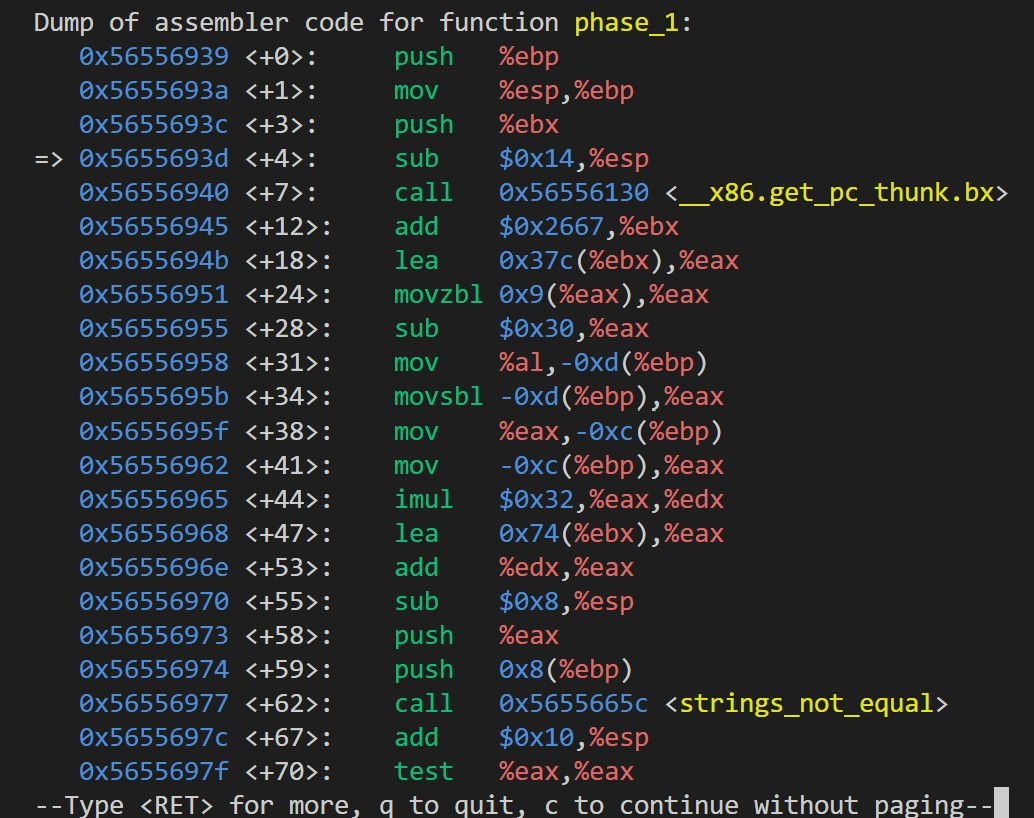
\includegraphics[scale=0.6]{images/3-1.jpg}
			\caption{phase 1}
			\label{fig3-1}
		\end{center}
	\end{figure}
	我们通过观察设置断点，然后查看eax的内容
	
	b *0x56556977
	
	c
	
	x/s eax
	
	\begin{figure}[H],
		\begin{center}
			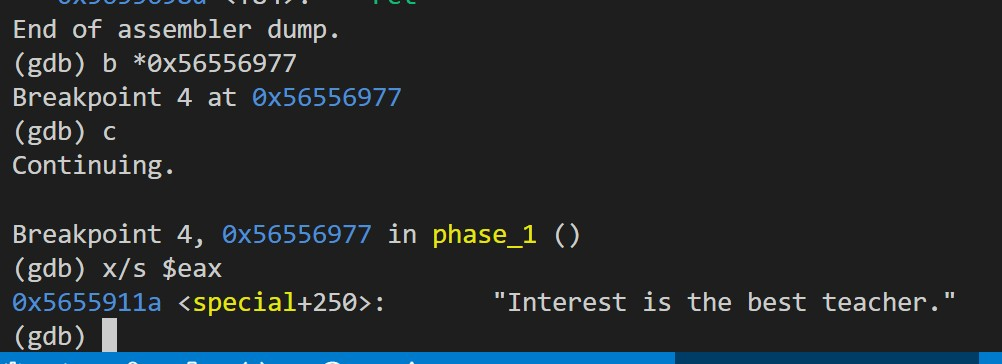
\includegraphics[scale=0.55]{images/3-2.jpg}
			\caption{phase 1}
			\label{fig3-2}
		\end{center}
	\end{figure}
	得到我们phase 1的答案：Interest is the best teacher.
	\subsubsection{阶段2：循环 phase\_2(char *input)}
	进入phase 2，随便输点数然后看看dias内容
	\begin{lstlisting}[style=commonCodeStyle, caption={phase2}, label={lst:3-1}]
		0x5655698e <+0>:     push   %ebp
		0x5655698f <+1>:     mov    %esp,%ebp
		0x56556991 <+3>:     push   %ebx
		=> 0x56556992 <+4>:     sub    $0x34,%esp
		0x56556995 <+7>:     call   0x56556130 <__x86.get_pc_thunk.bx>
		0x5655699a <+12>:    add    $0x2612,%ebx
		0x565569a0 <+18>:    mov    0x8(%ebp),%eax
		0x565569a3 <+21>:    mov    %eax,-0x2c(%ebp)
		0x565569a6 <+24>:    mov    %gs:0x14,%eax
		0x565569ac <+30>:    mov    %eax,-0xc(%ebp)
		0x565569af <+33>:    xor    %eax,%eax
		0x565569b1 <+35>:    sub    $0x8,%esp
		0x565569b4 <+38>:    lea    -0x24(%ebp),%eax
		0x565569b7 <+41>:    push   %eax
		0x565569b8 <+42>:    push   -0x2c(%ebp)
		0x565569bb <+45>:    call   0x565565c2 <read_six_numbers>
		0x565569c0 <+50>:    add    $0x10,%esp
		0x565569c3 <+53>:    mov    -0x24(%ebp),%eax
		0x565569c6 <+56>:    test   %eax,%eax
		0x565569c8 <+58>:    jns    0x565569cf <phase_2+65>
		0x565569ca <+60>:    call   0x56556907 <explode_bomb>
		0x565569cf <+65>:    mov    -0x24(%ebp),%edx
		--Type <RET> for more, q to quit, c to continue without paging--
		0x565569d2 <+68>:    lea    0x37c(%ebx),%eax
		0x565569d8 <+74>:    movzbl 0x9(%eax),%eax
		0x565569dc <+78>:    movsbl %al,%eax
		0x565569df <+81>:    sub    $0x30,%eax
		0x565569e2 <+84>:    cmp    %eax,%edx
		0x565569e4 <+86>:    je     0x565569eb <phase_2+93>
		0x565569e6 <+88>:    call   0x56556907 <explode_bomb>
		0x565569eb <+93>:    mov    -0x20(%ebp),%edx
		0x565569ee <+96>:    lea    0x37c(%ebx),%eax
		0x565569f4 <+102>:   movzbl 0x8(%eax),%eax
		0x565569f8 <+106>:   movsbl %al,%eax
		0x565569fb <+109>:   sub    $0x30,%eax
		0x565569fe <+112>:   cmp    %eax,%edx
		0x56556a00 <+114>:   je     0x56556a07 <phase_2+121>
		0x56556a02 <+116>:   call   0x56556907 <explode_bomb>
		0x56556a07 <+121>:   movl   $0x2,-0x28(%ebp)
		0x56556a0e <+128>:   jmp    0x56556a3a <phase_2+172>
		0x56556a10 <+130>:   mov    -0x28(%ebp),%eax
		0x56556a13 <+133>:   mov    -0x24(%ebp,%eax,4),%edx
		0x56556a17 <+137>:   mov    -0x28(%ebp),%eax
		0x56556a1a <+140>:   sub    $0x1,%eax
		0x56556a1d <+143>:   mov    -0x24(%ebp,%eax,4),%ecx
		0x56556a21 <+147>:   mov    -0x28(%ebp),%eax
		--Type <RET> for more, q to quit, c to continue without paging--
		0x56556a24 <+150>:   sub    $0x2,%eax
		0x56556a27 <+153>:   mov    -0x24(%ebp,%eax,4),%eax
		0x56556a2b <+157>:   add    %ecx,%eax
		0x56556a2d <+159>:   cmp    %eax,%edx
		0x56556a2f <+161>:   je     0x56556a36 <phase_2+168>
		0x56556a31 <+163>:   call   0x56556907 <explode_bomb>
		0x56556a36 <+168>:   addl   $0x1,-0x28(%ebp)
		0x56556a3a <+172>:   cmpl   $0x5,-0x28(%ebp)
		0x56556a3e <+176>:   jle    0x56556a10 <phase_2+130>
		0x56556a40 <+178>:   nop
		0x56556a41 <+179>:   mov    -0xc(%ebp),%eax
		0x56556a44 <+182>:   sub    %gs:0x14,%eax
		0x56556a4b <+189>:   je     0x56556a52 <phase_2+196>
		0x56556a4d <+191>:   call   0x56556f10 <__stack_chk_fail_local>
		0x56556a52 <+196>:   mov    -0x4(%ebp),%ebx
		0x56556a55 <+199>:   leave
		0x56556a56 <+200>:   ret
		
	\end{lstlisting}
	
	我们可以注意到
	
	取学号字符串中偏移量为 9 的字符 (即第10个字符)
	
	0x565569d8: movzbl 0x9(\%eax),\%eax  
	
	将字符转换为数字 ('0'的ASCII码是0x30)
	
	0x565569df: sub    \$0x30,\%eax      
	
	与输入的第 1 个数比较
	
	0x565569e2: cmp    \%eax,\%edx       
	
	然后
	
	取学号字符串中偏移量为 8 的字符 (即第9个字符)
	
	0x565569f4: movzbl 0x8(\%eax),\%eax  
	
	转换为数字
	
	0x565569fb: sub    \$0x30,\%eax      
	
	与输入的第 2 个数比较
	
	0x565569fe: cmp    \%eax,\%edx       
	
	以上，我们可以知道这是一个ficon数列，第一个数就是学号倒数第一个，第二个则是倒数第二个，所以对于我的学号来说，答案就是
	
	5 3 8 11 19 30
	
	\subsubsection{阶段3：条件分支 phase\_3(char *input)}
	\begin{lstlisting}[style=commonCodeStyle, caption={phase2}, label={lst:3-2}]
		0x56556a57 <+0>:     push   %ebp
		0x56556a58 <+1>:     mov    %esp,%ebp
		0x56556a5a <+3>:     push   %ebx
		=> 0x56556a5b <+4>:     sub    $0x34,%esp
		0x56556a5e <+7>:     call   0x56556130 <__x86.get_pc_thunk.bx>
		0x56556a63 <+12>:    add    $0x2549,%ebx
		0x56556a69 <+18>:    mov    0x8(%ebp),%eax
		0x56556a6c <+21>:    mov    %eax,-0x2c(%ebp)
		0x56556a6f <+24>:    mov    %gs:0x14,%eax
		0x56556a75 <+30>:    mov    %eax,-0xc(%ebp)
		0x56556a78 <+33>:    xor    %eax,%eax
		0x56556a7a <+35>:    movl   $0x0,-0x14(%ebp)
		0x56556a81 <+42>:    movl   $0x0,-0x10(%ebp)
		0x56556a88 <+49>:    lea    -0x18(%ebp),%eax
		0x56556a8b <+52>:    push   %eax
		0x56556a8c <+53>:    lea    -0x1c(%ebp),%eax
		0x56556a8f <+56>:    push   %eax
		0x56556a90 <+57>:    lea    -0x1c4c(%ebx),%eax
		0x56556a96 <+63>:    push   %eax
		0x56556a97 <+64>:    push   -0x2c(%ebp)
		0x56556a9a <+67>:    call   0x565560c0 <__isoc99_sscanf@plt>
		0x56556a9f <+72>:    add    $0x10,%esp
		--Type <RET> for more, q to quit, c to continue without paging--
		0x56556aa2 <+75>:    mov    %eax,-0x10(%ebp)
		0x56556aa5 <+78>:    cmpl   $0x1,-0x10(%ebp)
		0x56556aa9 <+82>:    jg     0x56556ab0 <phase_3+89>
		0x56556aab <+84>:    call   0x56556907 <explode_bomb>
		0x56556ab0 <+89>:    lea    0x37c(%ebx),%eax
		0x56556ab6 <+95>:    movzbl 0x7(%eax),%eax
		0x56556aba <+99>:    movsbl %al,%eax
		0x56556abd <+102>:   lea    -0x30(%eax),%edx
		0x56556ac0 <+105>:   mov    -0x1c(%ebp),%eax
		0x56556ac3 <+108>:   cmp    %eax,%edx
		0x56556ac5 <+110>:   je     0x56556acc <phase_3+117>
		0x56556ac7 <+112>:   call   0x56556907 <explode_bomb>
		0x56556acc <+117>:   mov    -0x1c(%ebp),%eax
		0x56556acf <+120>:   cmp    $0x9,%eax
		0x56556ad2 <+123>:   ja     0x56556b3c <phase_3+229>
		0x56556ad4 <+125>:   shl    $0x2,%eax
		0x56556ad7 <+128>:   mov    -0x1c44(%eax,%ebx,1),%eax
		0x56556ade <+135>:   add    %ebx,%eax
		0x56556ae0 <+137>:   jmp    *%eax
		0x56556ae2 <+139>:   movl   $0x32f,-0x14(%ebp)
		0x56556ae9 <+146>:   jmp    0x56556b41 <phase_3+234>
		0x56556aeb <+148>:   movl   $0x130,-0x14(%ebp)
		0x56556af2 <+155>:   jmp    0x56556b41 <phase_3+234>
		--Type <RET> for more, q to quit, c to continue without paging--
		0x56556af4 <+157>:   movl   $0x184,-0x14(%ebp)
		0x56556afb <+164>:   jmp    0x56556b41 <phase_3+234>
		0x56556afd <+166>:   movl   $0x28e,-0x14(%ebp)
		0x56556b04 <+173>:   jmp    0x56556b41 <phase_3+234>
		0x56556b06 <+175>:   movl   $0x11c,-0x14(%ebp)
		0x56556b0d <+182>:   jmp    0x56556b41 <phase_3+234>
		0x56556b0f <+184>:   movl   $0x201,-0x14(%ebp)
		0x56556b16 <+191>:   jmp    0x56556b41 <phase_3+234>
		0x56556b18 <+193>:   movl   $0x1a9,-0x14(%ebp)
		0x56556b1f <+200>:   jmp    0x56556b41 <phase_3+234>
		0x56556b21 <+202>:   movl   $0x374,-0x14(%ebp)
		0x56556b28 <+209>:   jmp    0x56556b41 <phase_3+234>
		0x56556b2a <+211>:   movl   $0x7b,-0x14(%ebp)
		0x56556b31 <+218>:   jmp    0x56556b41 <phase_3+234>
		0x56556b33 <+220>:   movl   $0x141,-0x14(%ebp)
		0x56556b3a <+227>:   jmp    0x56556b41 <phase_3+234>
		0x56556b3c <+229>:   call   0x56556907 <explode_bomb>
		0x56556b41 <+234>:   mov    -0x18(%ebp),%eax
		0x56556b44 <+237>:   cmp    %eax,-0x14(%ebp)
		0x56556b47 <+240>:   je     0x56556b4e <phase_3+247>
		0x56556b49 <+242>:   call   0x56556907 <explode_bomb>
		0x56556b4e <+247>:   nop
		0x56556b4f <+248>:   mov    -0xc(%ebp),%eax
		--Type <RET> for more, q to quit, c to continue without paging--
		0x56556b52 <+251>:   sub    %gs:0x14,%eax
		0x56556b59 <+258>:   je     0x56556b60 <phase_3+265>
		0x56556b5b <+260>:   call   0x56556f10 <__stack_chk_fail_local>
		0x56556b60 <+265>:   mov    -0x4(%ebp),%ebx
		0x56556b63 <+268>:   leave
		0x56556b64 <+269>:   ret
		
	\end{lstlisting}
	
	同理，我们可以看到
	
	0x56556ab6: movzbl 0x7(\%eax),\%eax    取学号字符串偏移量为 7 的字符 (即第8个字符)
	
	0x56556abd: lea    -0x30(\%eax),\%edx  将字符转换为数字 (减去 '0')
	
	0x56556ac0: mov    -0x1c(\%ebp),\%eax  取出你输入的第一个数 x
	
	0x56556ac3: cmp    \%eax,\%edx         比较 x 和学号第8个字符
	
	则第一个数是0
	
	0x56556ad7: mov    -0x1c44(\%eax,\%ebx,1),\%eax  ; 查表跳转
	
	0x56556ae0: jmp    *\%eax                      ; 跳转到对应 case
	
	0x56556ae2: movl   \$0x32f,-0x14(\%ebp) ; 将预期结果设为 0x32f
	
	0x56556ae9: jmp    0x56556b41         ; 跳转到结尾比较
	
	因此可以算出第二个数是815
	\begin{figure}[H],
		\begin{center}
			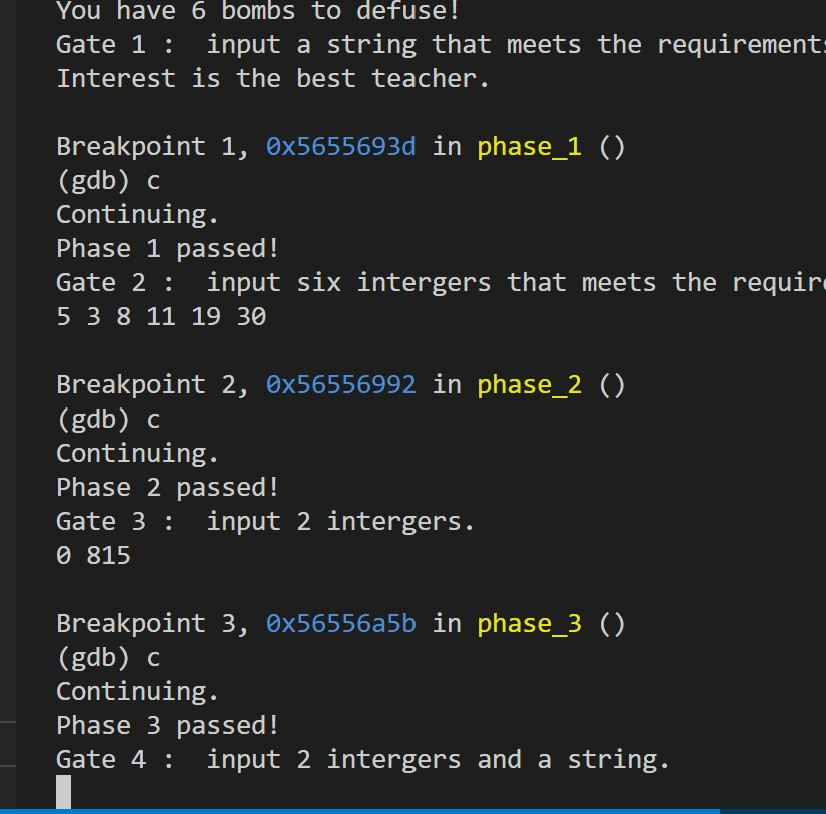
\includegraphics[scale=0.6]{images/3-3.jpg}
			\caption{phase 3}
			\label{fig3-3}
		\end{center}
	\end{figure}
	
	\subsection{体会}
	本次实验通过逆向分析 Linux 环境下的 ELF 可执行文件（Binary Bomb），深入实践了机器级语言的表示与调试技术。本次实验不仅提升了我的反汇编阅读能力，更重要的是培养了「逆向思维」。在没有源码的情况下，通过寄存器状态和内存数据推断程序意图，这种能力对于理解系统底层安全和程序优化具有重要意义。
	
	\section{缓冲区溢出攻击}
	\subsection{实验目的与要求}
	通过分析一个程序（称为“缓冲区炸弹”）的构成和运行逻辑，加深对理论课中关于程序的机器级表示、函数调用规则、栈结构等方面知识点的理解，增强反汇编、跟踪、分析、调试等能力，加深对缓冲区溢出攻击原理、方法与防范等方面知识的理解和掌握；
	
	实验环境：Ubuntu，GCC，GDB等
	
	
	\subsection{实验内容}
	\subsubsection{缓冲区溢出攻击}
	程序运行过程中，需要输入特定的字符串，使得程序达到期望的运行效果。
	
	对一个可执行程序“bufbomb” 实施一系列缓冲区溢出攻击(buffer overflow attacks)，也就是设法通过造成缓冲区溢出来改变该程序的运行内存映像(例如将专门设计的字节序列插入到栈中特定内存位置)和行为，以
	
	实现实验预定的目标。bufbomb 目标程序在运行时使用函数 getbuf读入一个字符串。根据不同的任务，学生生成相应的攻击字符串。
	
	实验中需要针对目标可执行程序bufbomb,分别完成多个难度递增的缓冲区溢出攻击(完成的顺序没有固定要求)。按从易到难的顺序，这些难度级分别命名为smoke (level 1)、fizz (level 2)。 
	
	\subsubsection{第1级 smoke}
	正常情况下，getbuf函数运行结束，执行最后的ret指令时，将取出保存于栈帧中的返回（断点）地址并跳转至它继续执行（test函数中调用getbuf处）。要求将返回地址的值改为本级别实验的目标smoke函数的首条指令的地址， getbuf函数返回时，跳转到smoke函数执行，即达到了实验的目标。
	\subsubsection{第2级 fizz}
	要求getbuf函数运行结束后，转到 fizz函数处执行。与smoke的差别是，fizz函数有一个参数。 fizz函数中比较了参数val 与 全局变量cookie的值，只有两者相同（要正确打印val）才能达到目标。
	
	\subsection{实验记录及问题回答}
	我们在生成好了文件之后用gdb查看下内容
	\subsubsection{第1级 smoke}
	\begin{figure}[H],
		\begin{center}
			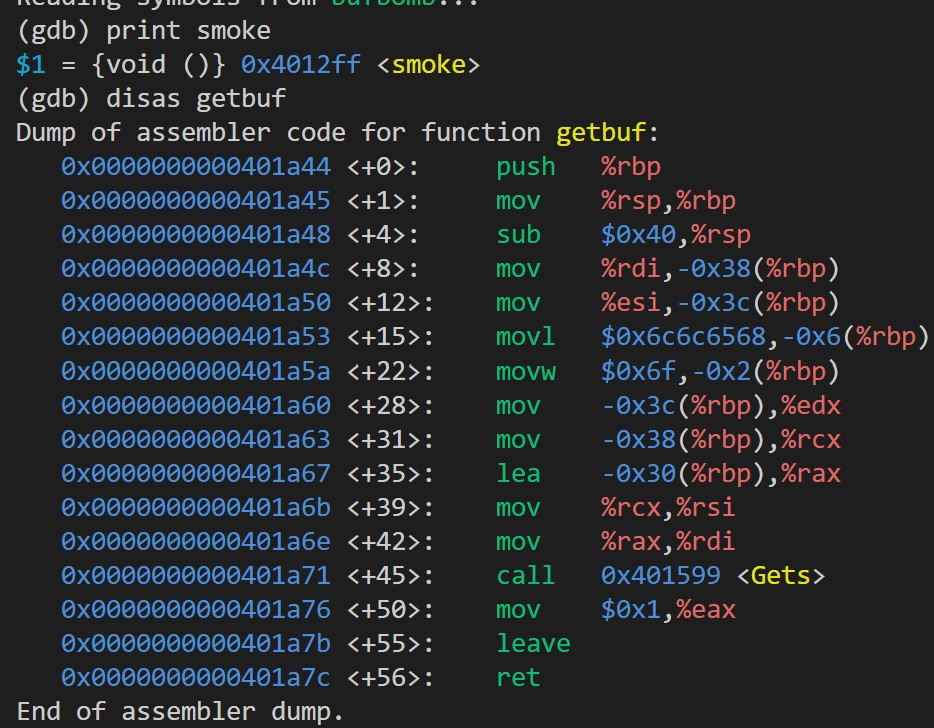
\includegraphics[scale=0.6]{images/4-2.jpg}
			\caption{smoke}
			\label{fig4-2}
		\end{center}
	\end{figure}
	目标地址 (smoke)：
	
	从截图中可以看到 print smoke 的结果是：0x4012ff。
	
	这就是我们想让程序跳转去执行的地方。
	
	缓冲区距离 (Offset)：
	
	从 disas getbuf 截图中看到指令：lea -0x30(\%rbp),\%rax。
	
	这说明缓冲区 (Buffer) 开始于 rbp - 0x30 (即 rbp - 48)。
	
	返回地址 (Return Address) 存储在 rbp + 8 的位置（这是 64 位系统的标准）。
	
	计算距离：
	
	从 Buffer (-48) 到 rbp (0) 需要填充 48 个字节。
	
	覆盖旧的 rbp (8 个字节) 需要再填充 8 个字节。
	
	总共需要填充：48 + 8 = 56 个字节 的垃圾数据，才能刚好摸到返回地址。
	
	因此我们写入
	
	00 00 00 00 00 00 00 00 00 00 00 00 00 00 00 00
	00 00 00 00 00 00 00 00 00 00 00 00 00 00 00 00
	00 00 00 00 00 00 00 00 00 00 00 00 00 00 00 00
	00 00 00 00 00 00 00 00
	ff 12 40 00 00 00 00 00
	
	然后运行，可以实现攻击了
	
	\begin{figure}[H],
		\begin{center}
			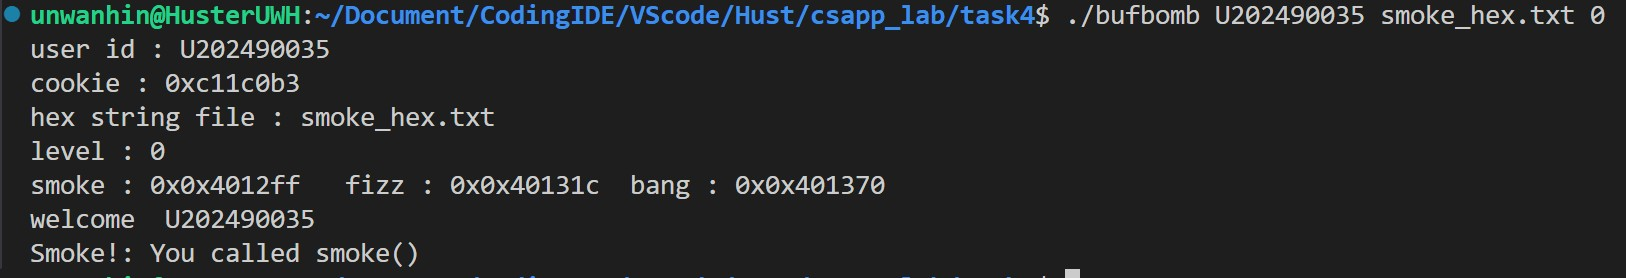
\includegraphics[scale=0.6]{images/4-1.jpg}
			\caption{smoke}
			\label{fig4-1}
		\end{center}
	\end{figure}
	\begin{figure}[H],
		\begin{center}
			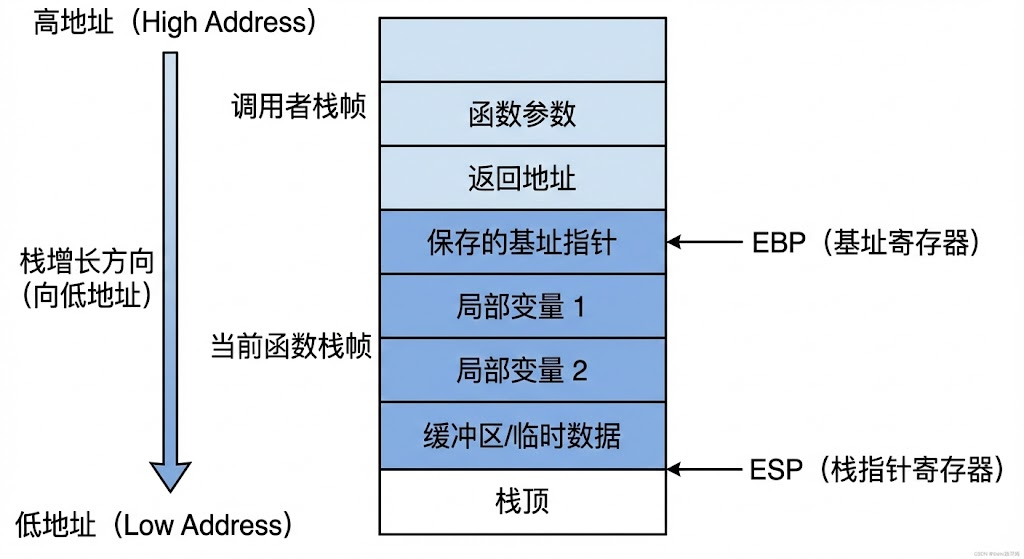
\includegraphics[scale=0.3]{images/4-3.jpg}
			\caption{graph}
			\label{fig4-3}
		\end{center}
	\end{figure}
	
	\subsubsection{第2级 fizz}
	首先我们观察fizz，可以看到0x401327和0x40132d一个Cookie 放入 eax另一个比较 eax 和 rbp - 4 的值，因此我们不从头开始执行 fizz，而是直接跳转到 0x401327。 只要我们能控制 rbp，让 rbp - 4 的内存位置刚好存放着我们的 Cookie，就可能会成功
	\begin{figure}[H],
		\begin{center}
			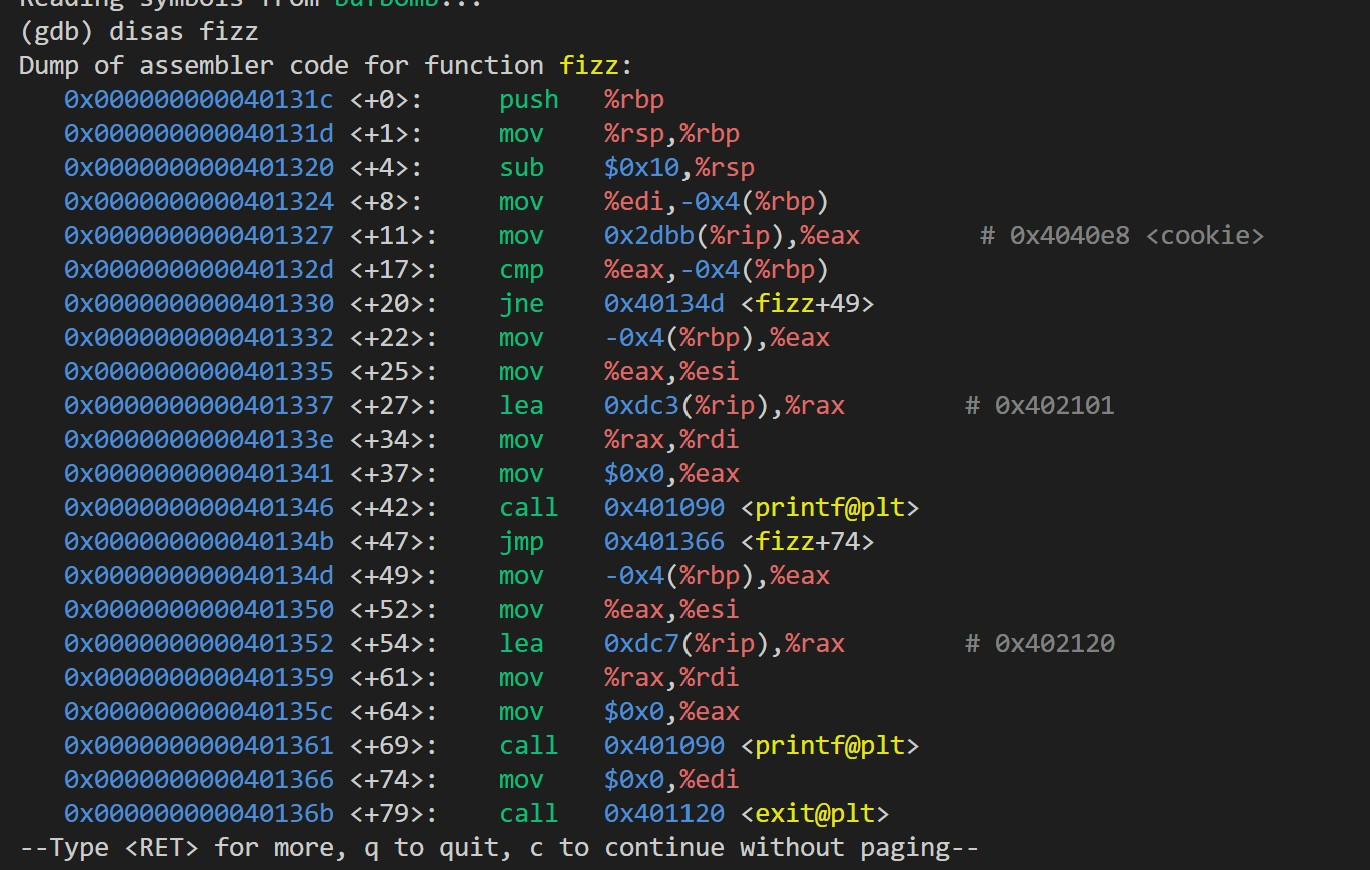
\includegraphics[scale=0.6]{images/4-4.jpg}
			\caption{fizz}
			\label{fig4-4}
		\end{center}
	\end{figure}
	
	
	现在我们拥有通关 Level 1 (Fizz) 的所有数据：
	
	Cookie (密码): 0xc11c0b3
	
	目标地址 (Fizz 中间): 0x401327
	
	缓冲区地址: 0x7fffffffc4d0
	
	我们的目标是让 fizz 执行 cmp eax, -0x4(rbp) 时，内存 -0x4(rbp) 里刚好是我们的 Cookie。
	
	因此我们就可以建立txt文本如下
	
	b3 c0 11 0c 00 00 00 00 00 00 00 00 00 00 00 00
	00 00 00 00 00 00 00 00 00 00 00 00 00 00 00 00
	00 00 00 00 00 00 00 00 00 00 00 00 00 00 00 00
	d4 c4 ff ff ff 7f 00 00
	27 13 40 00 00 00 00 00
	
	\begin{figure}[H],
		\begin{center}
			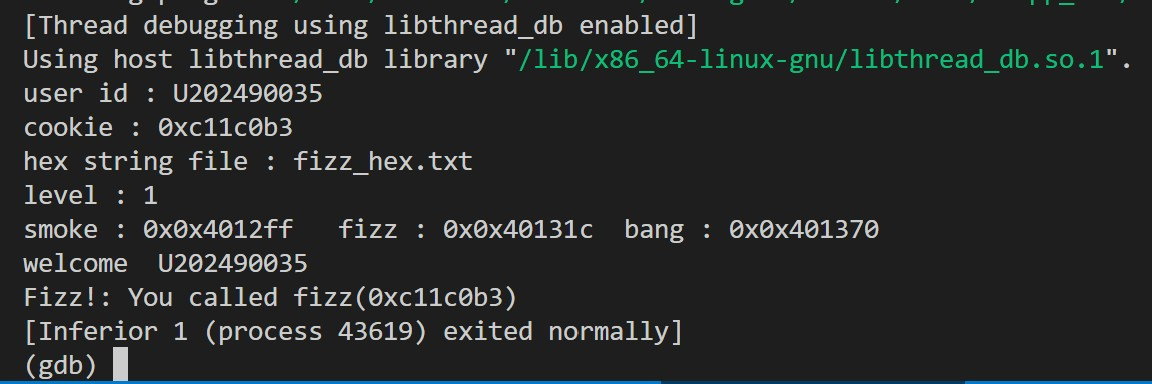
\includegraphics[scale=0.6]{images/4-5.jpg}
			\caption{fizz}
			\label{fig4-5}
		\end{center}
	\end{figure}
	\subsection{体会}
	本次「缓冲区溢出攻击」实验是我第一次从攻击者的视角审视程序安全，这与以往编写防御性代码的体验截然不同。通过对 bufbomb 程序的逆向分析与攻击，我对计算器系统底层机制有了更深刻的理解：
	
	1. 栈帧结构的具象化理解 在理论课上，我们学习了栈帧由返回地址、保存的帧指针（Saved RBP）和局部变量组成。但在本次实验中，我必须通过 GDB 的 disas 指令精确计算缓冲区起始地址到返回地址的偏移量（48字节缓冲区 + 8字节 RBP）。这让我真正理解了「数据」与「控制信息」在栈上是如何紧密相邻存放的，正是这种相邻关系导致了缓冲区溢出漏洞的产生。
	
	2. 数据流控制与栈迁移技术 在 Level 1 的破解中，我遇到了一个难题：需要在跳转的同时传递参数 cookie。由于无法直接修改寄存器，我分析汇编代码发现程序会读取 rbp-0x4 处的值。我采用了栈迁移（Stack Pivoting）的思想，通过将栈上的 Saved RBP 覆盖为伪造的地址，成功欺骗了程序，使其去我预设的地方读取参数。这让我体会到，攻击不仅仅是简单的地址覆盖，更需要对汇编逻辑进行精妙的利用。
	
	\section{链接炸弹拆除}
	\subsection{实验目的与要求}
	通过修改给定的可复位位的目标文件（链接炸弹），加深对可复位位目标文件格式、目标文件的生成、以及链接的理论知识的理解。
	
	实验环境：Ubuntu
	
	工具：GCC、GDB、readelf、hexdump、hexedit、od等。
	
	
	\subsection{实验内容}
	\subsubsection{链接炸弹的拆除}
	在二进制层面，逐步修改构成目标程序“linkbomb”的多个二进制模块（“.o文件”），然后链接生成可执行程序，要求可执行程序运行能得到指定的效果。修改目标包括可复位位目标文件中的数据、机器指令、复位位记录等。
	\subsubsection{第1关 数据节的修改}
	修改二进制可复位位目标文件 phase1.o 的数据节中的内容（不允许修改其他节），使其与main.o链接后，生成的执行程序，可以输出自己的学号。
	\subsubsection{第2关 简单的机器指令修改}
	修改二进制可复位位目标文件 phase2.o 的代码节中的内容（不允许修改其他节），使其与main.o链接后，生成的执行程序。在phase\_2.c 中，有一个静态函数 myfunc( ) ，要求在 do\_phase 函数中调用myfunc( )，显示信息myfunc is called!。
	
	static void myfunc()
	
	{	printf("myfunc is called!\n");   }
	
	\subsubsection{第3关 有参数的函数调用的机器指令修改}
	修改二进制可复位位目标文件 phase3.o 的代码节中的内容（不允许修改其他节），使其与main.o链接后，生成的执行程序。在phase\_3.c 中，有一个静态函数 static void myfunc(int offset) ，要求在 do\_phase函数中调用myfunc(pos )，将do\_phase的参数pos直接传递myfunc，显示相应的信息。
	\subsubsection{第4关 有局部变量的机器指令修改}
	修改二进制可复位位目标文件 phase4.o 的代码节中的内容（不允许修改其他节），使其与main.o链接后，生成的执行程序。在phase\_4.c 中，有一个静态函数 static void myfunc(char *s) ，要求在 do\_phase 函数中调用myfunc(s )，显示出自己的学号。
	\subsubsection{第5关 复位位表的修改}
	修改二进制可复位位目标文件 phase5.o 的复位位节中的内容（不允许修改代码节和数据节），使其与main.o链接后，生成的执行程序运行时，显示Class Name :  Computer Foundation.  Teacher Name : Xu Xiangyang。
	\subsubsection{第6关 强弱符号}
	不准修改 main.c 和phase6.o，通过增补一个文件，使得程序链接后，能够输出自己的学号。
	
	#gcc  -no-pie  -o  linkbomb6   main.o  phase6.o phase6\_patch.o
	
	\subsubsection{第7关 只读数据节的修改}
	修改 phase7.o 中只读数据节（不准修改代码节），使其与main.o链接后，能够输出自己的学号。
	
	\subsection{实验记录及问题回答}
	
	\subsubsection{第1关 数据节的修改}
	这里我们用下好的hexedit，然后打开二进制查看，之后在abcde...的地方改为我们的学号就好了
	\begin{figure}[H],
		\begin{center}
			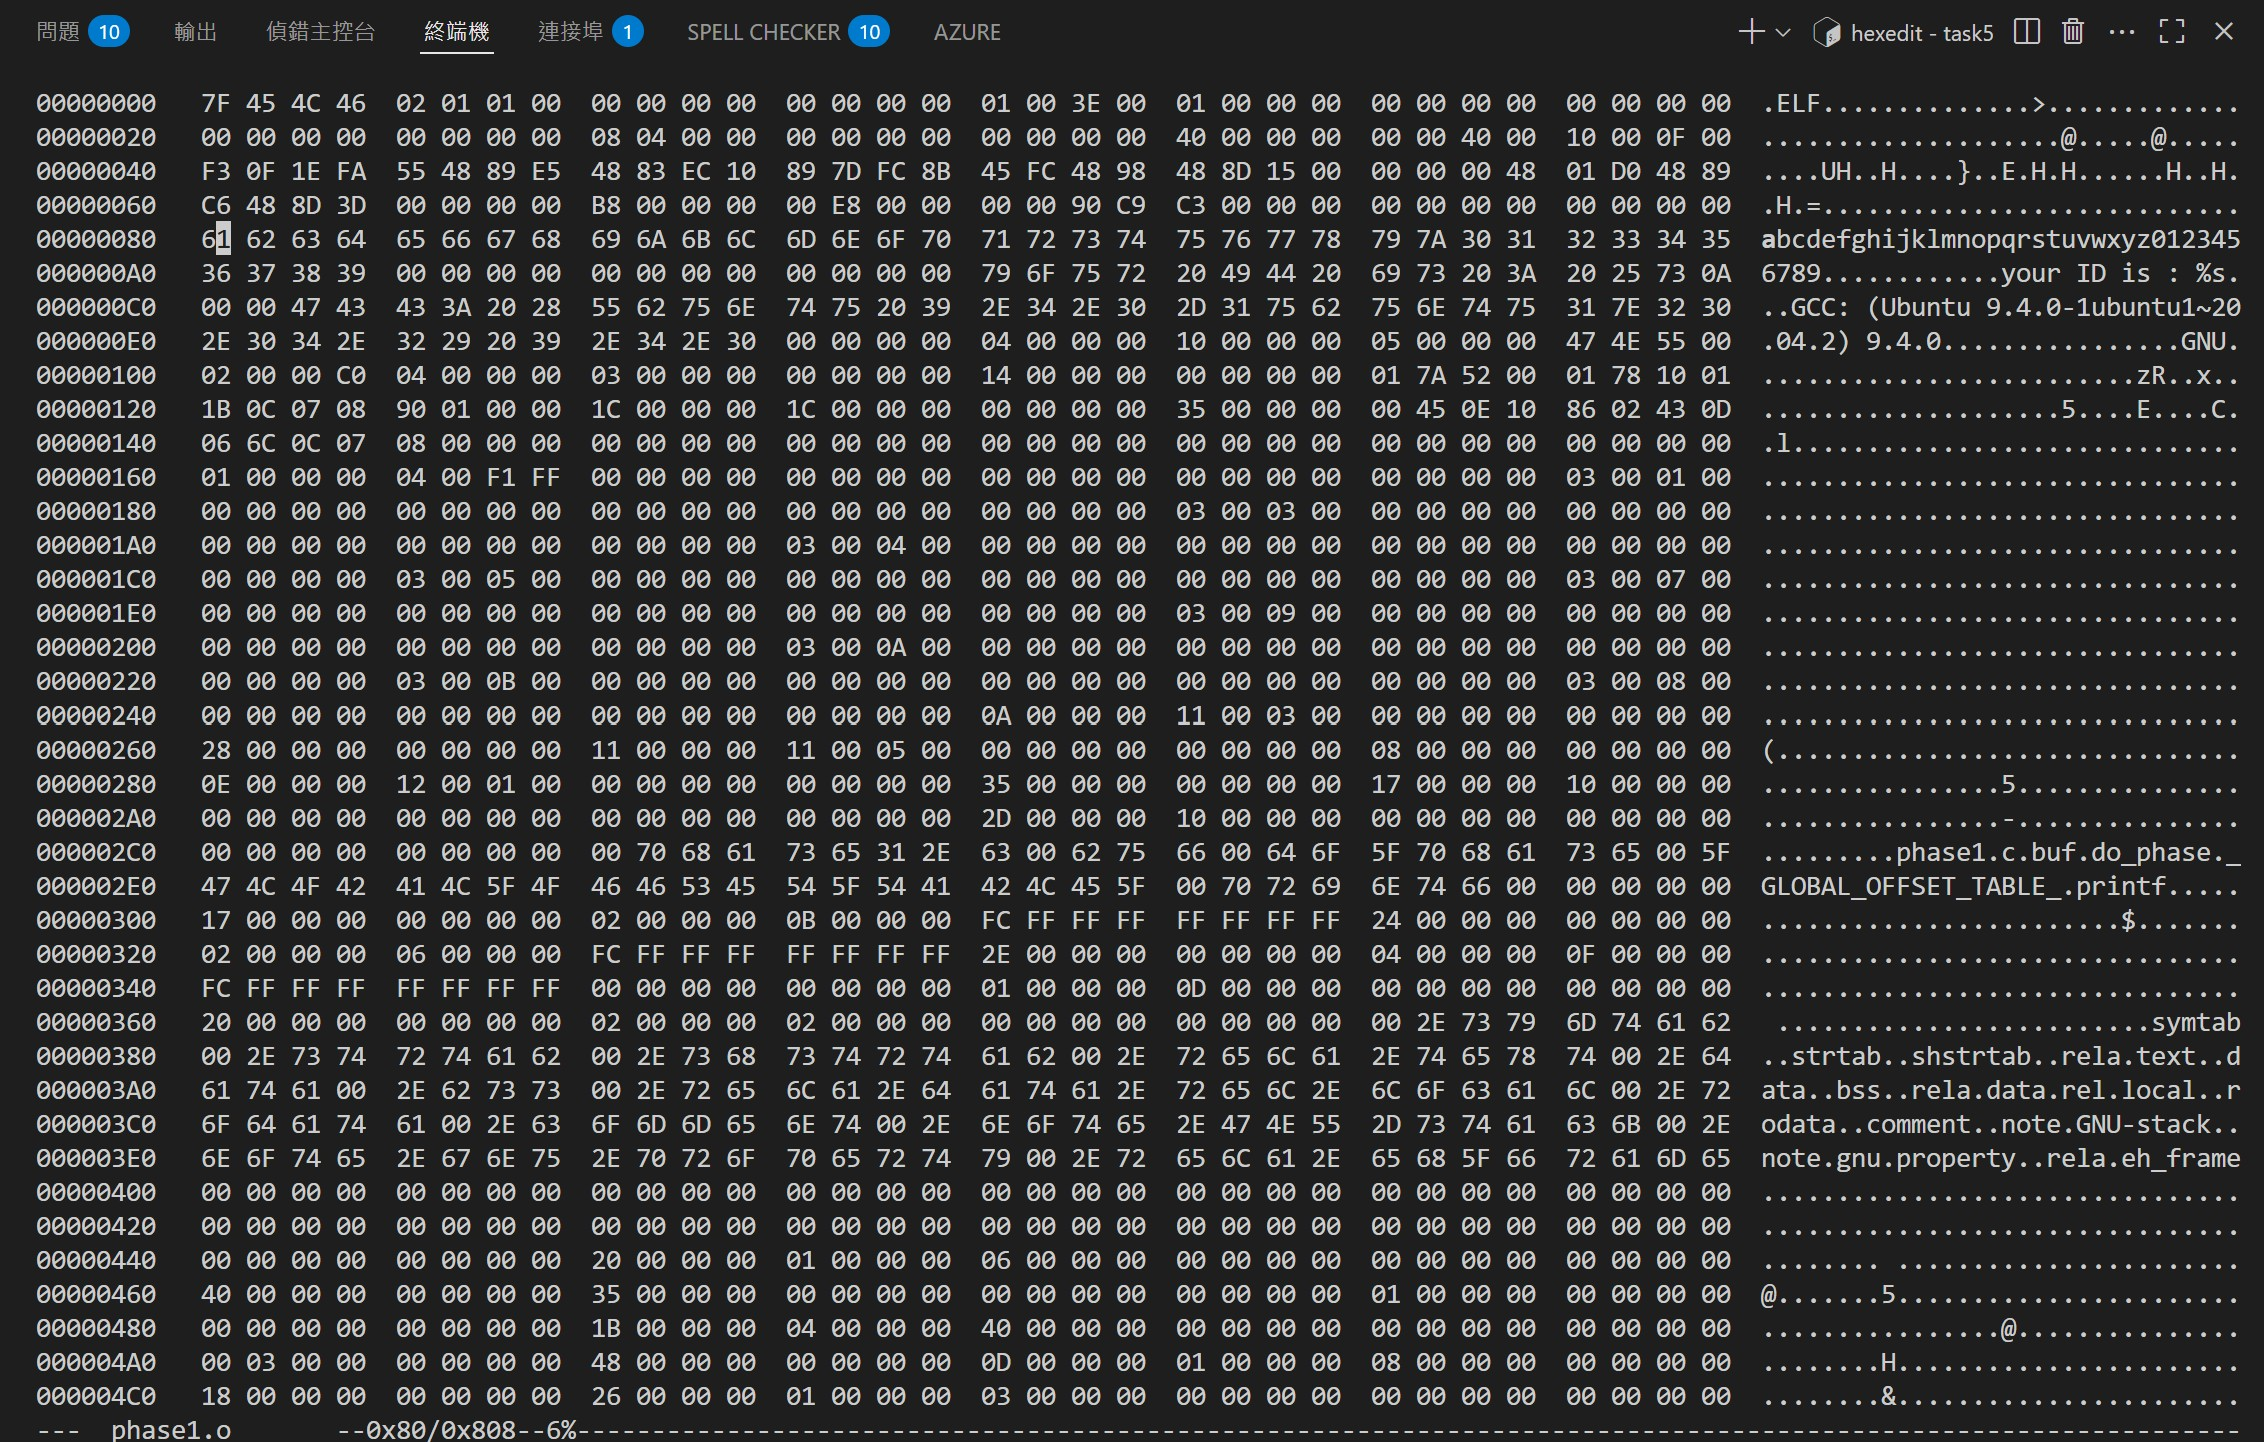
\includegraphics[scale=0.3]{images/5-1.jpg}
			\caption{1}
			\label{fig5-1}
		\end{center}
	\end{figure}
	
	\begin{figure}[H],
		\begin{center}
			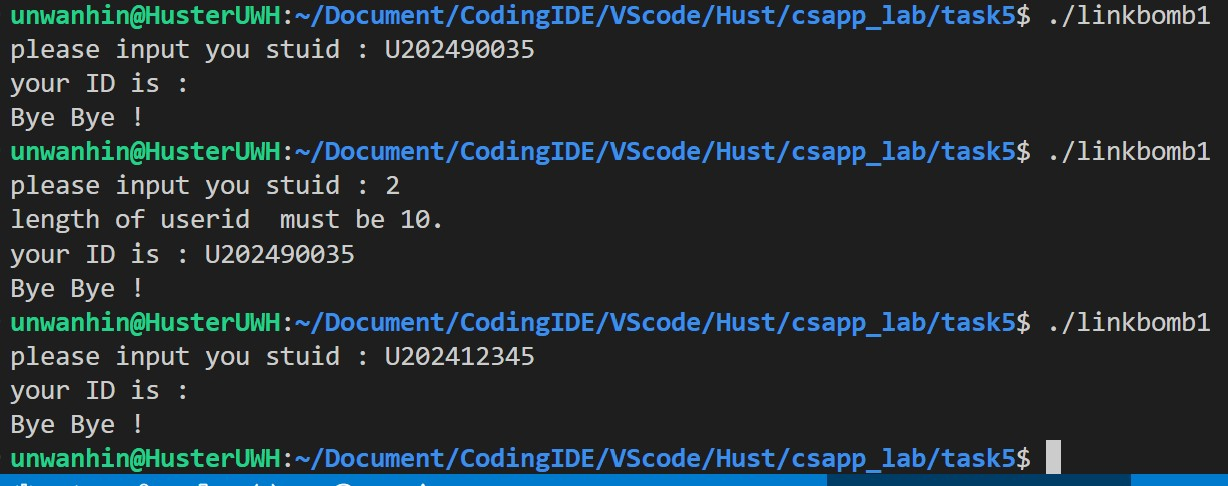
\includegraphics[scale=0.6]{images/5-2.jpg}
			\caption{1}
			\label{fig5-2}
		\end{center}
	\end{figure}
	\subsubsection{第2关 简单的机器指令修改}
	我们必须先知道 myfunc 和 do\_phase 在内存中的相对位置，才能计算跳转的距离。
	\begin{figure}[H],
		\begin{center}
			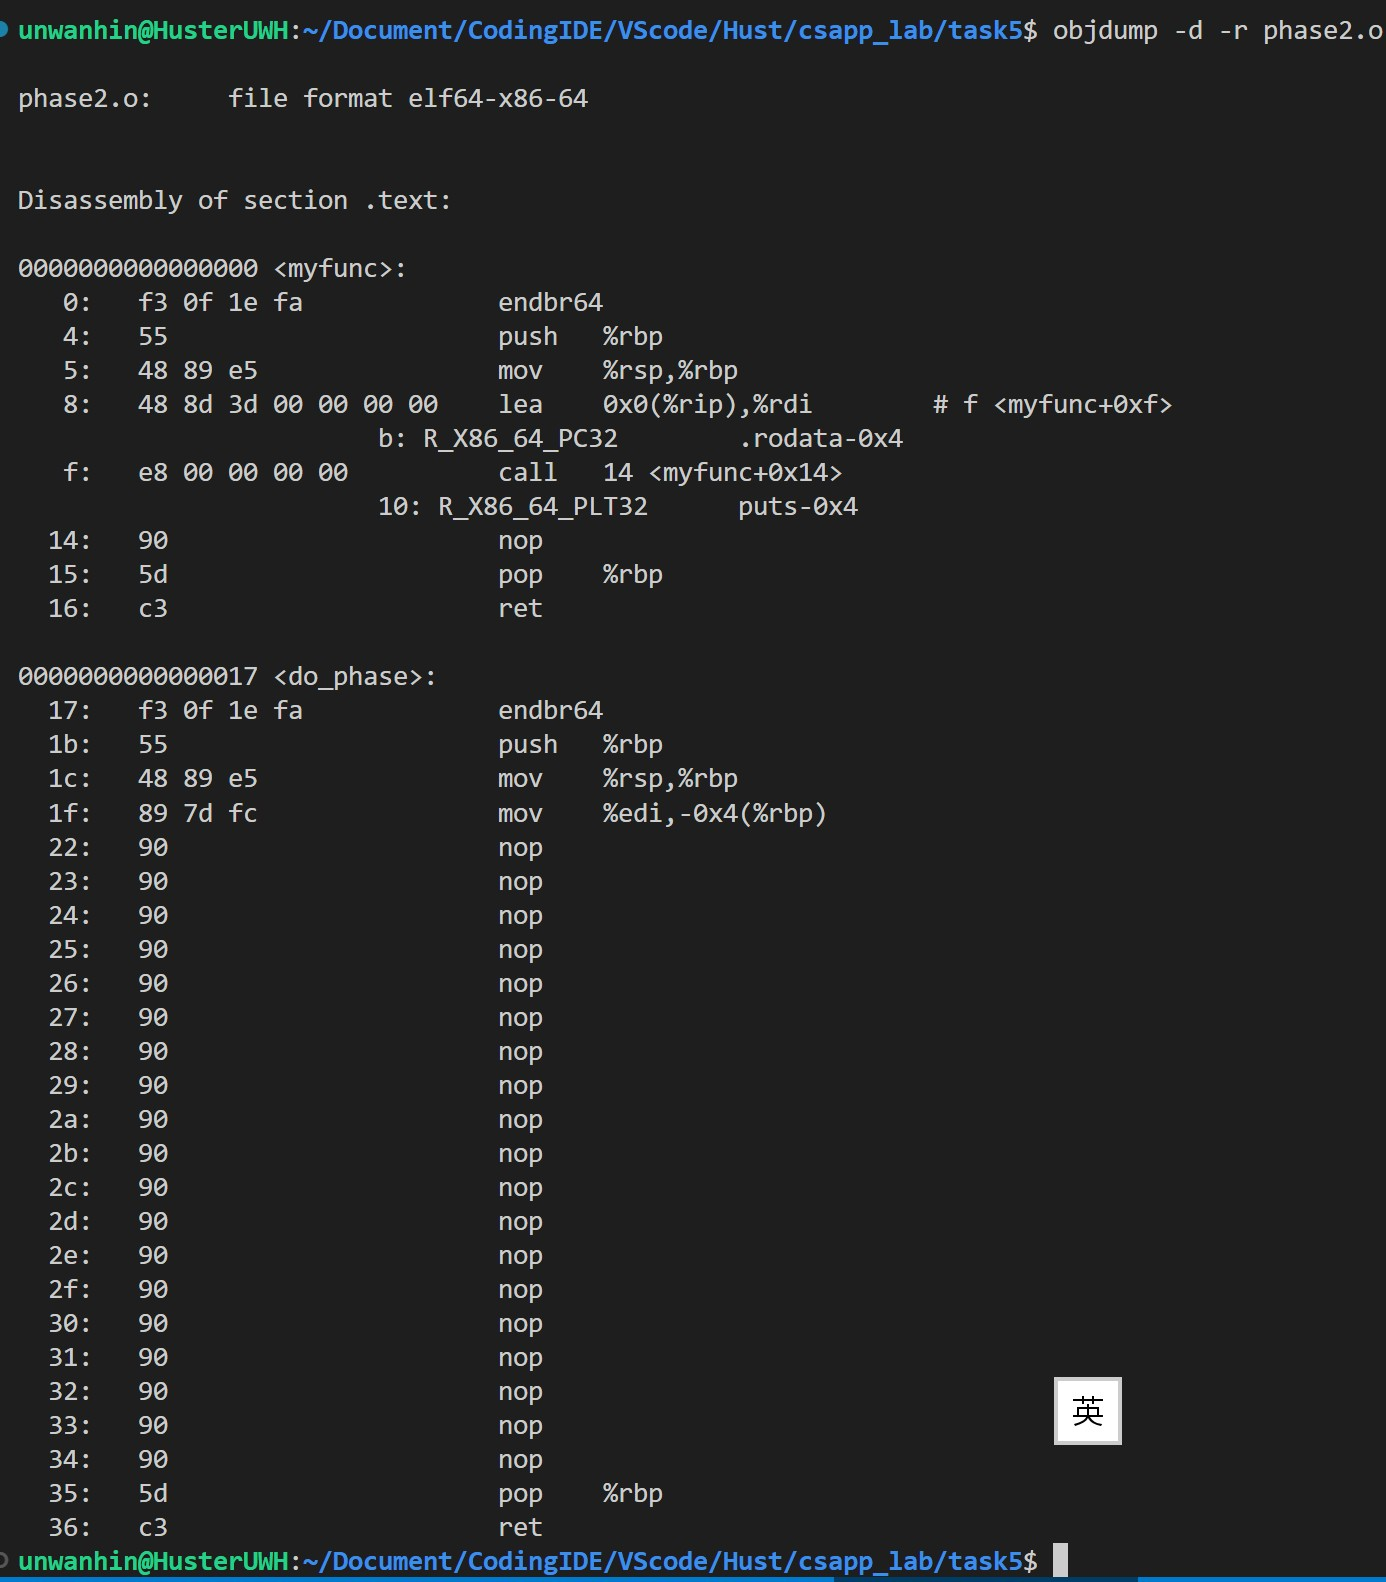
\includegraphics[scale=0.6]{images/5-3.jpg}
			\caption{2}
			\label{fig5-3}
		\end{center}
	\end{figure}
	89 7D FC 是 mov \%edi,-0x4(\%rbp) 的指令。后面紧跟着的一大堆 90 就是我们要改的地方。我们改为E8 D9 FF FF FF，改完之后就发成能call函数出来了
	\begin{figure}[H]
		\begin{center}
			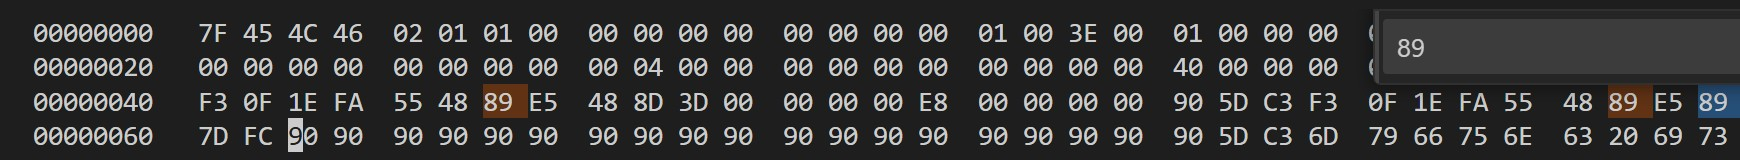
\includegraphics[scale=0.6]{images/5-4.jpg}
			\caption{2}
			\label{fig5-4}
		\end{center}
	\end{figure}
	\begin{figure}[H]
		\begin{center}
			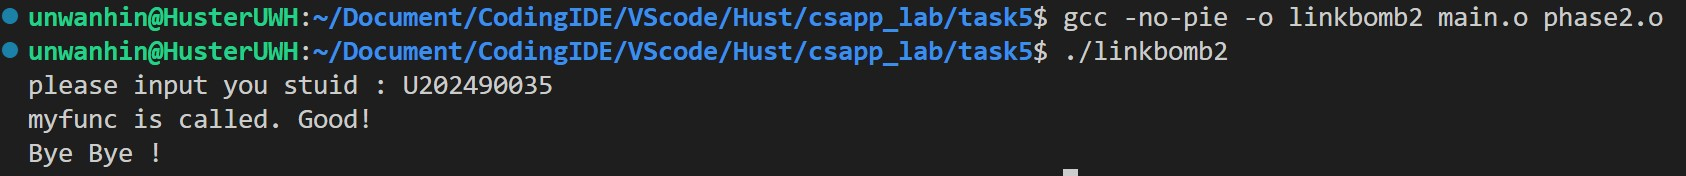
\includegraphics[scale=0.6]{images/5-5.jpg}
			\caption{2}
			\label{fig5-5}
		\end{center}
	\end{figure}
	
	\subsubsection{第3关 有参数的函数调用的机器指令修改}
	我们来破解 Phase 3。这一关的目标是让 do\_phase 调用 myfunc(pos)，这涉及到 参数传递。
	
	我们需要在 0x33 的位置写入两步操作：
	
	准备参数：把保存在堆栈里的 pos 取出来，重新放回 \%edi 寄存器（这是 myfunc 要读取的地方）。。
	
	调用函数：执行 call myfunc。
	\begin{lstlisting}[style=commonCodeStyle, caption={phase3}, label={lst:5-1}]
		phase3.o:     file format elf64-x86-64
		
		
		Disassembly of section .text:
		
		0000000000000000 <myfunc>:
		0:   f3 0f 1e fa             endbr64
		4:   55                      push   %rbp
		5:   48 89 e5                mov    %rsp,%rbp
		8:   48 83 ec 10             sub    $0x10,%rsp
		c:   89 7d fc                mov    %edi,-0x4(%rbp)
		f:   8b 45 fc                mov    -0x4(%rbp),%eax
		12:   89 c6                   mov    %eax,%esi
		14:   48 8d 3d 00 00 00 00    lea    0x0(%rip),%rdi        # 1b <myfunc+0x1b>
		17: R_X86_64_PC32       .rodata-0x4
		1b:   b8 00 00 00 00          mov    $0x0,%eax
		20:   e8 00 00 00 00          call   25 <myfunc+0x25>
		21: R_X86_64_PLT32      printf-0x4
		25:   90                      nop
		26:   c9                      leave
		27:   c3                      ret
		
		0000000000000028 <do_phase>:
		28:   f3 0f 1e fa             endbr64
		2c:   55                      push   %rbp
		2d:   48 89 e5                mov    %rsp,%rbp
		30:   89 7d fc                mov    %edi,-0x4(%rbp)
		33:   90                      nop
		34:   90                      nop
		35:   90                      nop
		36:   90                      nop
		37:   90                      nop
		38:   90                      nop
		39:   90                      nop
		3a:   90                      nop
		3b:   90                      nop
		3c:   90                      nop
		3d:   90                      nop
		3e:   90                      nop
		3f:   90                      nop
		40:   90                      nop
		41:   90                      nop
		42:   90                      nop
		43:   90                      nop
		44:   90                      nop
		45:   90                      nop
		46:   90                      nop
		47:   90                      nop
		48:   90                      nop
		49:   5d                      pop    %rbp
		4a:   c3                      ret
		
	\end{lstlisting}
	\begin{figure}[H]
		\begin{center}
			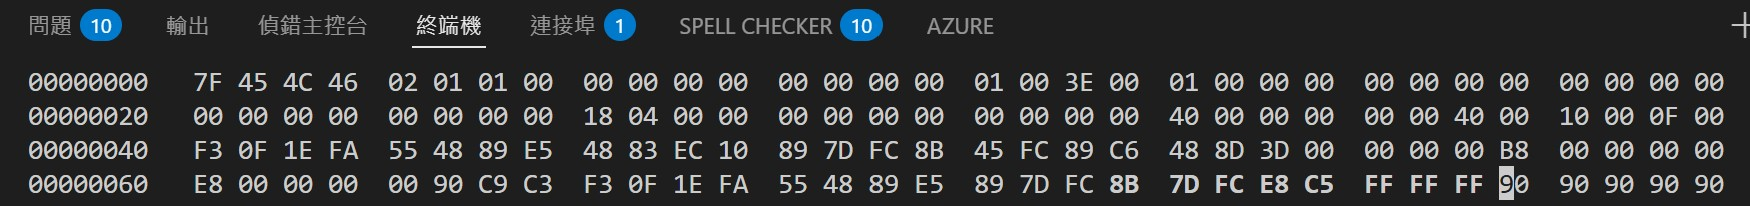
\includegraphics[scale=0.6]{images/5-6.jpg}
			\caption{3}
			\label{fig5-6}
		\end{center}
	\end{figure}
	\begin{figure}[H]
		\begin{center}
			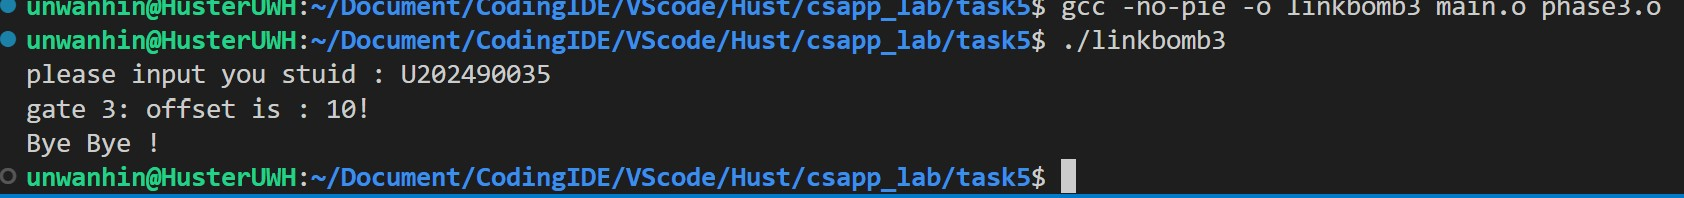
\includegraphics[scale=0.6]{images/5-7.jpg}
			\caption{3}
			\label{fig5-7}
		\end{center}
	\end{figure}
	\subsubsection{第4关 有局部变量的机器指令修改}
	
	\begin{lstlisting}[style=commonCodeStyle, caption={phase4}, label={lst:5-2}]
		phase4.o:     file format elf64-x86-64
		
		
		Disassembly of section .text:
		
		0000000000000000 <myfunc>:
		0:   f3 0f 1e fa             endbr64
		4:   55                      push   %rbp
		5:   48 89 e5                mov    %rsp,%rbp
		8:   48 83 ec 10             sub    $0x10,%rsp
		c:   48 89 7d f8             mov    %rdi,-0x8(%rbp)
		10:   48 8b 45 f8             mov    -0x8(%rbp),%rax
		14:   48 89 c6                mov    %rax,%rsi
		17:   48 8d 3d 00 00 00 00    lea    0x0(%rip),%rdi        # 1e <myfunc+0x1e>
		1a: R_X86_64_PC32       .rodata-0x4
		1e:   b8 00 00 00 00          mov    $0x0,%eax
		23:   e8 00 00 00 00          call   28 <myfunc+0x28>
		24: R_X86_64_PLT32      printf-0x4
		28:   90                      nop
		29:   c9                      leave
		2a:   c3                      ret
		
		000000000000002b <do_phase>:
		2b:   f3 0f 1e fa             endbr64
		2f:   55                      push   %rbp
		30:   48 89 e5                mov    %rsp,%rbp
		33:   48 83 ec 30             sub    $0x30,%rsp
		37:   89 7d dc                mov    %edi,-0x24(%rbp)
		3a:   64 48 8b 04 25 28 00    mov    %fs:0x28,%rax
		41:   00 00 
		43:   48 89 45 f8             mov    %rax,-0x8(%rbp)
		47:   31 c0                   xor    %eax,%eax
		49:   48 b8 55 32 30 32 32    movabs $0x3332313232303255,%rax
		50:   31 32 33 
		53:   48 89 45 ed             mov    %rax,-0x13(%rbp)
		57:   66 c7 45 f5 34 35       movw   $0x3534,-0xb(%rbp)
		5d:   c6 45 f7 00             movb   $0x0,-0x9(%rbp)
		61:   90                      nop
		62:   90                      nop
		63:   90                      nop
		64:   90                      nop
		65:   90                      nop
		66:   90                      nop
		67:   90                      nop
		68:   90                      nop
		69:   90                      nop
		6a:   90                      nop
		6b:   90                      nop
		6c:   90                      nop
		6d:   90                      nop
		6e:   90                      nop
		6f:   90                      nop
		70:   90                      nop
		71:   90                      nop
		72:   90                      nop
		73:   90                      nop
		74:   90                      nop
		75:   48 8b 45 f8             mov    -0x8(%rbp),%rax
		79:   64 48 33 04 25 28 00    xor    %fs:0x28,%rax
		80:   00 00 
		82:   74 05                   je     89 <do_phase+0x5e>
		84:   e8 00 00 00 00          call   89 <do_phase+0x5e>
		85: R_X86_64_PLT32      __stack_chk_fail-0x4
		89:   c9                      leave
		8a:   c3                      ret
	\end{lstlisting}
	我们需要在 0x61 处写入以下逻辑：
	
	计算学号地址：把 \%rbp - 0x13 的有效地址 (Effective Address) 加载到 \%rdi 寄存器中。
	
	指令：lea -0x13(\%rbp), \%rdi
	
	调用函数：call myfunc。
	
	找到 do\_phase 里的特征序列：C6 45 F7 00 90 90...
	
	从第一个 90 开始，依次输入：
	
	48 8D 7D ED E8 96 FF FF FF
	
	\begin{figure}[H]
		\begin{center}
			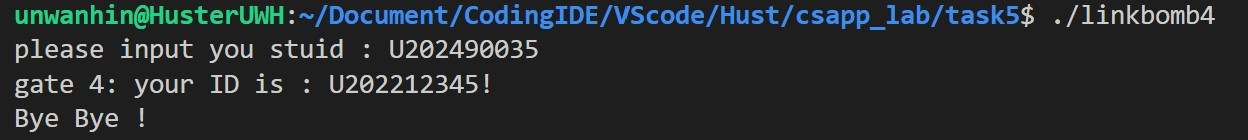
\includegraphics[scale=0.6]{images/5-8.jpg}
			\caption{4}
			\label{fig5-8}
		\end{center}
	\end{figure}
	
	
	\subsubsection{第5关 复位位表的修改}
	预期输出：Class Name : Computer Foundation. Teacher Name : Xu Xiangyang
	
	\begin{lstlisting}[style=commonCodeStyle, caption={phase5}, label={lst:5-3}]
		phase5.o:     file format elf64-x86-64
		
		
		Disassembly of section .text:
		
		0000000000000000 <do_phase>:
		0:   f3 0f 1e fa             endbr64
		4:   55                      push   %rbp
		5:   48 89 e5                mov    %rsp,%rbp
		8:   48 83 ec 10             sub    $0x10,%rsp
		c:   89 7d fc                mov    %edi,-0x4(%rbp)
		f:   48 8d 35 00 00 00 00    lea    0x0(%rip),%rsi        # 16 <do_phase+0x16>
		12: R_X86_64_PC32       originalclass-0x4
		16:   48 8d 3d 00 00 00 00    lea    0x0(%rip),%rdi        # 1d <do_phase+0x1d>
		19: R_X86_64_PC32       .rodata-0x4
		1d:   b8 00 00 00 00          mov    $0x0,%eax
		22:   e8 00 00 00 00          call   27 <do_phase+0x27>
		23: R_X86_64_PLT32      printf-0x4
		27:   48 8d 35 00 00 00 00    lea    0x0(%rip),%rsi        # 2e <do_phase+0x2e>
		2a: R_X86_64_PC32       originalteacher-0x4
		2e:   48 8d 3d 00 00 00 00    lea    0x0(%rip),%rdi        # 35 <do_phase+0x35>
		31: R_X86_64_PC32       .rodata+0xb
		35:   b8 00 00 00 00          mov    $0x0,%eax
		3a:   e8 00 00 00 00          call   3f <do_phase+0x3f>
		3b: R_X86_64_PLT32      printf-0x4
		3f:   90                      nop
		40:   90                      nop
		41:   90                      nop
		42:   90                      nop
		43:   90                      nop
		44:   90                      nop
		45:   90                      nop
		46:   90                      nop
		47:   90                      nop
		48:   90                      nop
		49:   90                      nop
		4a:   90                      nop
		4b:   90                      nop
		4c:   90                      nop
		4d:   90                      nop
		4e:   90                      nop
		4f:   90                      nop
		50:   90                      nop
		51:   90                      nop
		52:   90                      nop
		53:   90                      nop
		54:   90                      nop
		55:   c9                      leave
		56:   c3                      ret
	\end{lstlisting}
	字符串位置分析
	正确字符串：
	
	0x00: "Computer Foundation"
	
	0x20: "Xu Xiangyang"
	
	错误字符串：
	
	0x40: "c programming" (对应符号 originalclass)
	
	0x60: "ma" (对应符号 originalteacher)
	
	复位位表 .rela.text 在文件中的起始偏移量是 0x3f8。 每一条记录占 24 字节 (Offset 8字节 + Info 8字节 + Addend 8字节)。我们只需要修改 Addend。
	
	对此我们只要把408和450的FC改成BC就能成功了
	
	\begin{figure}[H]
		\begin{center}
			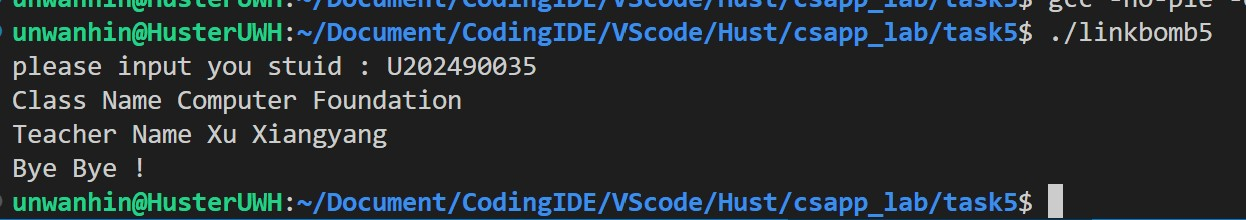
\includegraphics[scale=0.6]{images/5-9.jpg}
			\caption{5}
			\label{fig5-9}
		\end{center}
	\end{figure}
	
	
	\subsubsection{第6关 强弱符号}
	我们需要知道 phase6.o 里哪个函数是「弱」的，或者哪个函数被调用但未定义。
	\begin{figure}[H]
		\begin{center}
			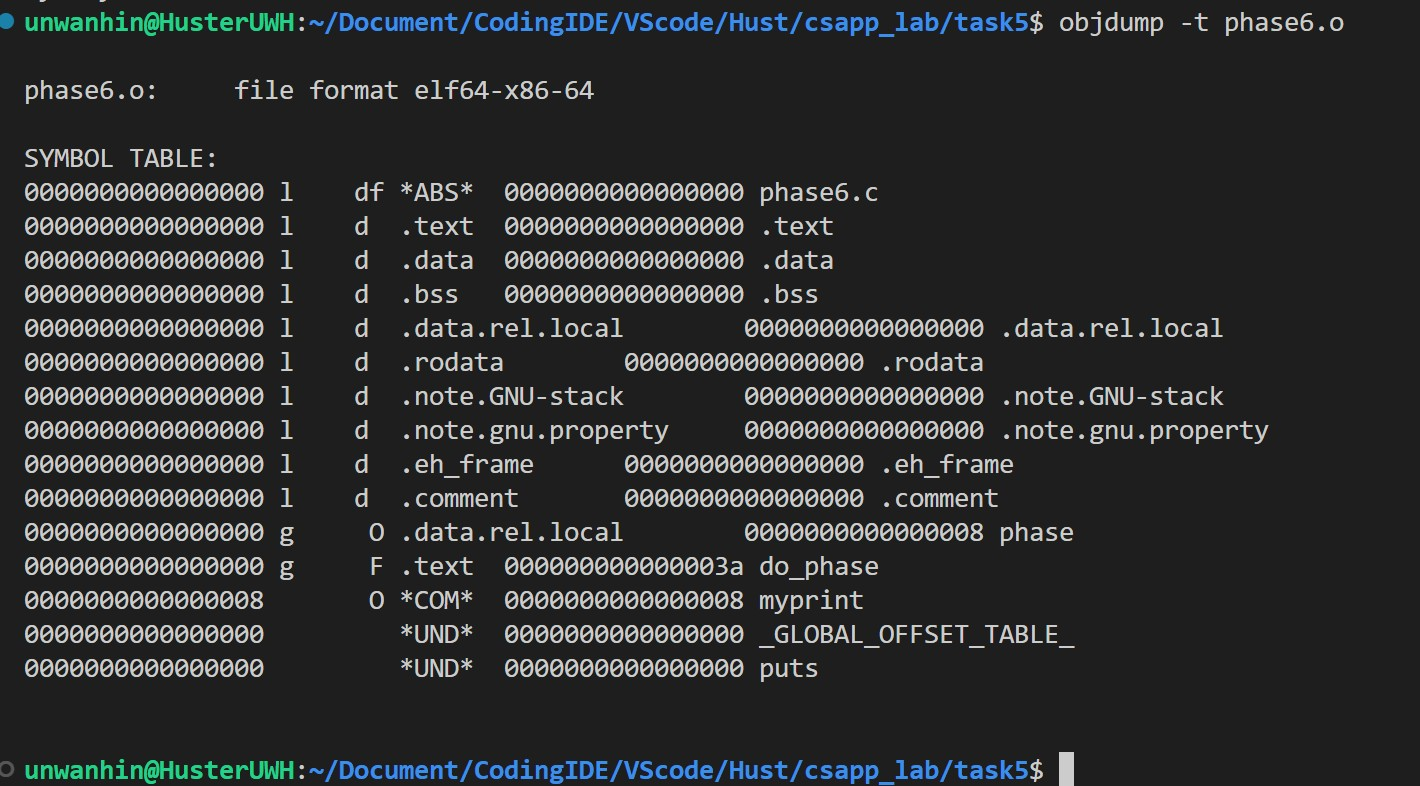
\includegraphics[scale=0.6]{images/5-10.jpg}
			\caption{6}
			\label{fig5-10}
		\end{center}
	\end{figure}
	发现：
	
	符号：myprint
	
	类型：O (Object，表示它是一个变量，不是函数)
	
	位置：*COM* (Common Section)
	
	大小：8 (字节，正好是一个 64 位指针的大小)
	\begin{lstlisting}[style=commonCodeStyle, caption={phase6}, label={lst:5-4}]
		#include <stdio.h>
		
		void print_my_id() {
			printf("U202490035\n");
		}
		
		void (*myprint)() = print_my_id;
	\end{lstlisting}
	
	\begin{figure}[H]
		\begin{center}
			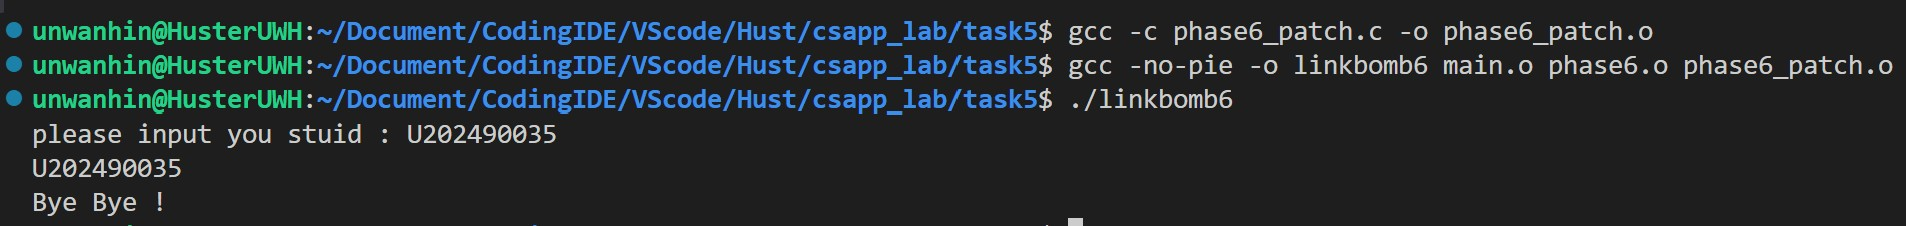
\includegraphics[scale=0.6]{images/5-11.jpg}
			\caption{6}
			\label{fig5-11}
		\end{center}
	\end{figure}
	\subsubsection{第7关 只读数据节的修改}
	phase7.o 里硬编码了一个别人的学号
	
	目标：把它改成U202490035。
	\begin{figure}[H]
		\begin{center}
			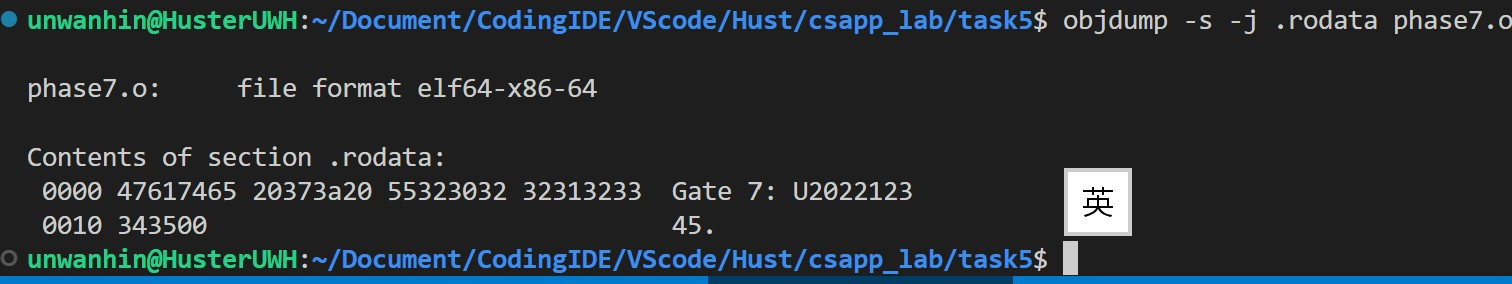
\includegraphics[scale=0.6]{images/5-12.jpg}
			\caption{7}
			\label{fig5-12}
		\end{center}
	\end{figure}
	我们像phase1那样改就好了
	\begin{figure}[H]
		\begin{center}
			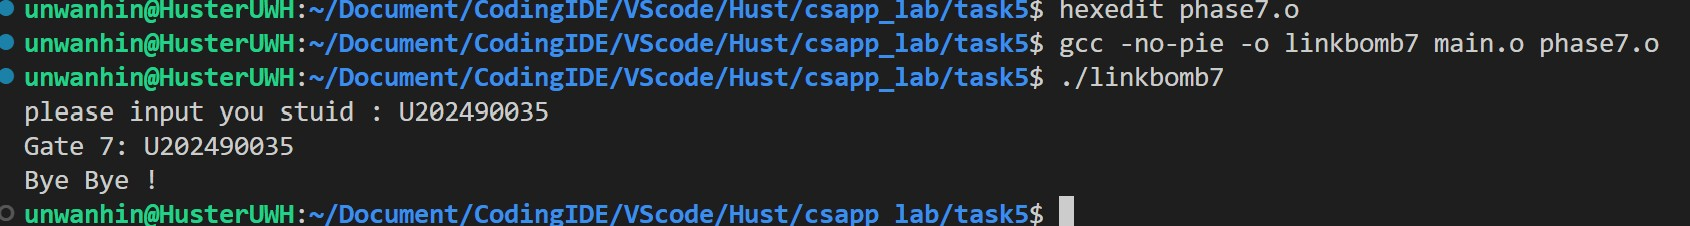
\includegraphics[scale=0.6]{images/5-13.jpg}
			\caption{13}
			\label{fig5-13}
		\end{center}
	\end{figure}
	
	
	\subsection{体会}
	本次「链接炸弹」实验通过对 ELF 可复位位目标文件的逆向分析与直接修改，让我深入理解了链接器的工作原理以及计算器程序的二进制表示。
	
	对 ELF 文件结构的立体认识 以往对 .text（代码节）、.data（数据节）、.rodata（只读数据节）的理解仅停留在概念层面。通过 Phase 1 和 Phase 7 的实践，我直接使用十六进制编辑器修改了数据节和只读数据节的内容，直观地看到了变量与常量在二进制文件中的存储形式，理解了为什么 C 语言字符串需要 \0 截断以及 ASCII 码的底层映像。
	
	机器级指令的编码与修改 Phase 2、3、4 是本次实验的难点，也是收获最大的部分。我学会了如何手动构造机器指令
	
	复位位与符号解析的本质 Phase 5 和 Phase 6 展示了链接器最核心的功能。
	
	复位位表：在 Phase 5 中，我没有修改一行代码，仅通过修改 .rela.text 中的 Addend（加数），就改变了指针引用的目标字符串。这让我明白了链接器是如何将代码中的占位符修正为最终的内存地址的。
	
	\section{ARM指令系统的理解}
	\subsection{实验目的与要求}
	通过在ARM虚拟环境下调试执行程序，了解 ARM的指令系统。
	
	实验环境：ARM 虚拟实验环境  QEMU
	
	工具：gcc, gdb 等
	
	
	\subsection{实验内容}
	程序及操作方法 见 <ARM实验任务.pdf>
	\subsubsection{任务1、C与汇编的混合编程}
	\subsubsection{任务2、内存拷贝及优化实验}
	查阅《ISA\_A64\_xml\_A\_profile-2023-09.pdf》，指出10条不同指令（存数、取数、算术运算、转移指令、函数调用等都应覆盖）的功能。
	
	\subsection{实验记录及问题回答}
	好的我们根据实验要求，自己先随便写一个冒泡排序的代码
	\begin{lstlisting}[style=commonCodeStyle, caption={task1.cpp}, label={lst:7-1}]
		#include <stdio.h>
		void print_array(int arr[], int n) {
			for (int i = 0; i < n; i++) {
				printf("%d ", arr[i]);
			}
			printf("\n");
		}
		
		int main() {
			int arr[] = {64, 34, 25, 12, 22, 11, 90, 5};
			int n = sizeof(arr) / sizeof(arr[0]);
			
			printf("[ARM Experiment] Bubble Sort Demo\n");
			printf("Original array: ");
			print_array(arr, n);
			
			int i, j, temp;
			for (i = 0; i < n - 1; i++) {
				for (j = 0; j < n - i - 1; j++) {
					if (arr[j] > arr[j + 1]) {
						temp = arr[j];
						arr[j] = arr[j + 1];
						arr[j + 1] = temp;
					}
				}
			}
			
			printf("Sorted array:   ");
			print_array(arr, n);
			return 0;
		}
	\end{lstlisting}
	
	我们先是生成arm文件aarch64-linux-gnu-gcc -g -static bubble.c -o bubble\_arm	，然后file bubble\_arm
	\begin{figure}[H]
		\begin{center}
			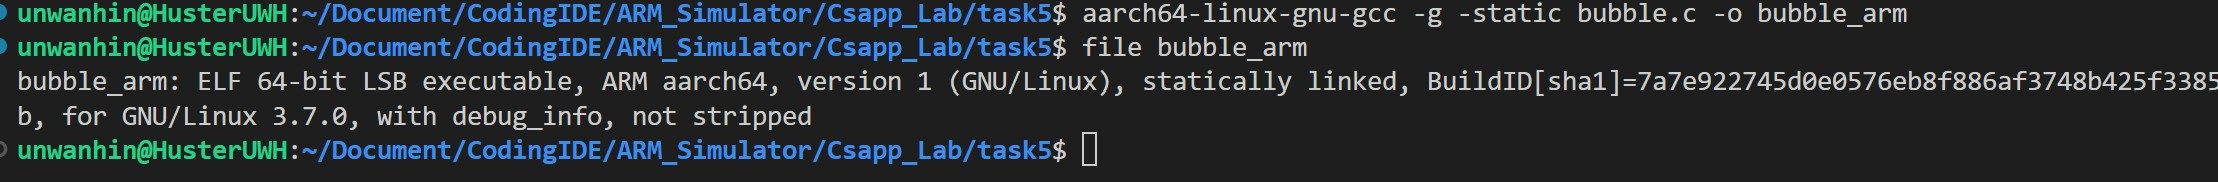
\includegraphics[scale=0.55]{images/6-1.jpg}
			\caption{arm}
			\label{fig6-1}
		\end{center}
	\end{figure}
	从 file 命令输出可以看到，生成的文件是 ELF 64-bit LSB executable, ARM aarch64，说明成功生成了 ARM 架构的可执行文件，无法在 x86 机器上直接运行。因此我们需要arm模拟工具
	
	qemu-aarch64 ./bubble\_arm
	\begin{figure}[H]
		\begin{center}
			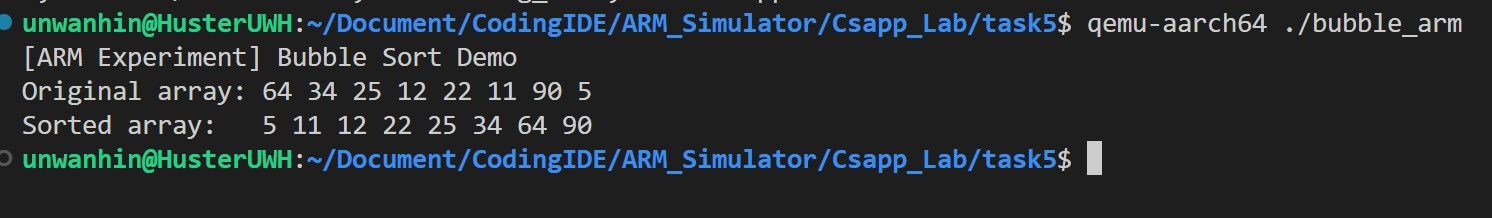
\includegraphics[scale=0.6]{images/6-2.jpg}
			\caption{arm}
			\label{fig6-2}
		\end{center}
	\end{figure}
	
	程序正确执行，数组被成功排序，证明交叉编译与模拟环境工作正常。
	
	\begin{figure}[H]
		\begin{center}
			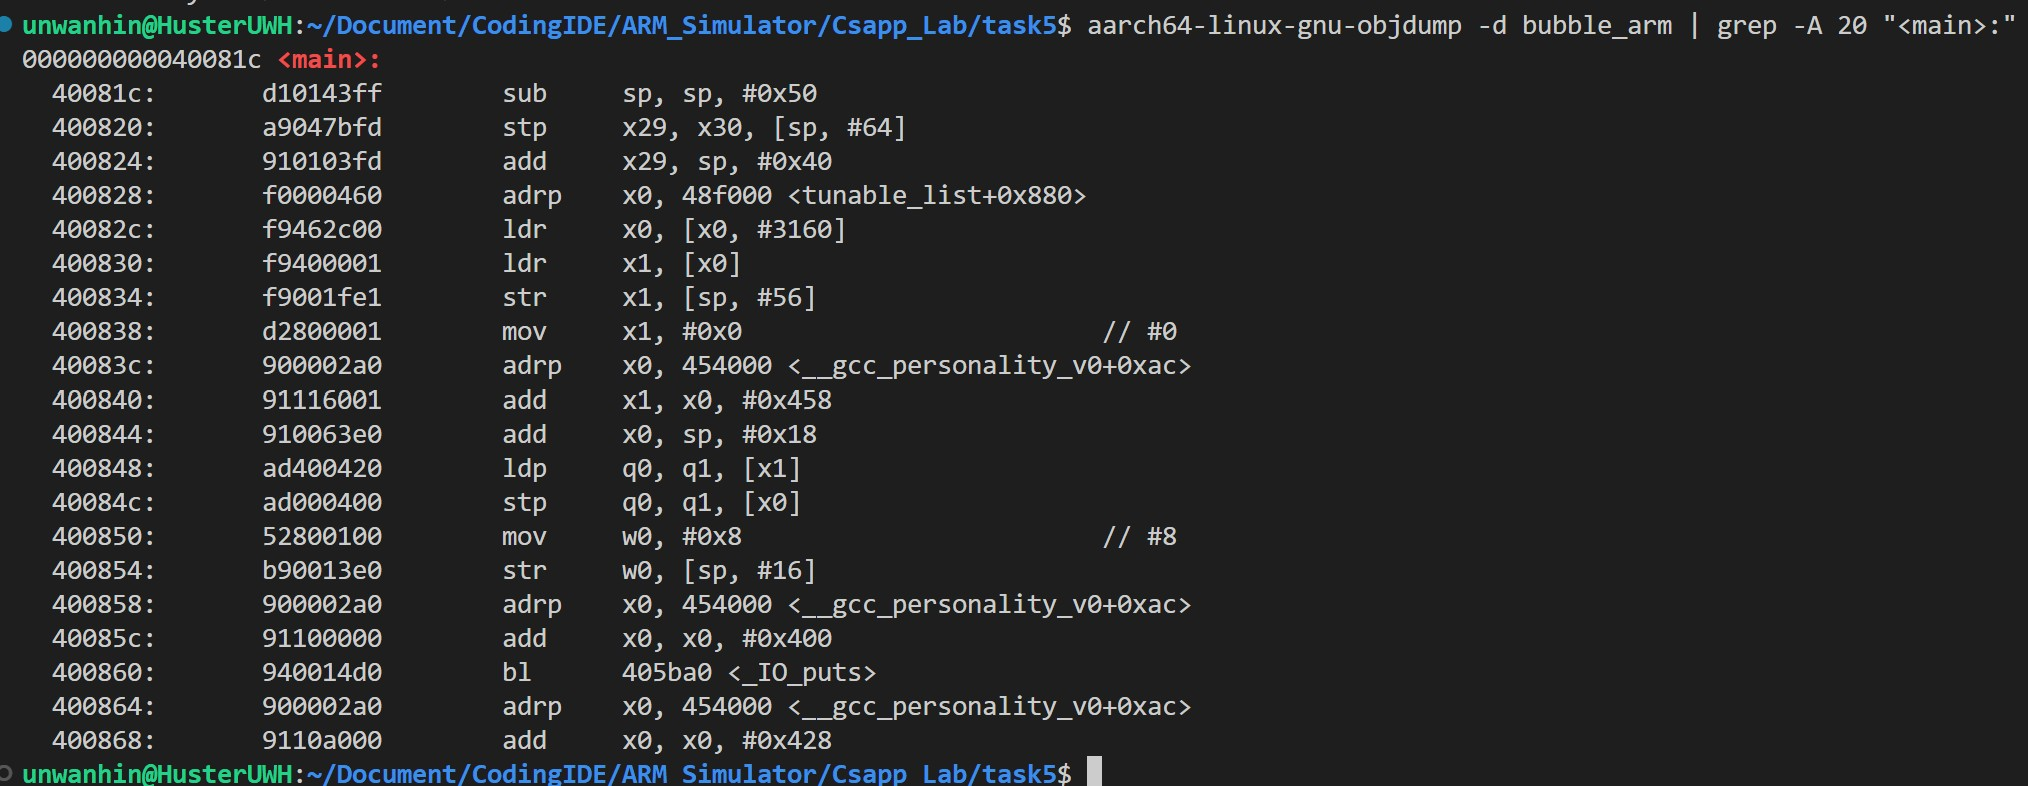
\includegraphics[scale=0.6]{images/6-3.jpg}
			\caption{arm}
			\label{fig6-3}
		\end{center}
	\end{figure}
	
	观察汇编代码，可以看到与 x86 显著不同的特征：
	
	寄存器使用 x29, x30（分别对应 FP 和 LR）以及 w0, w1 等通用寄存器。
	
	大量使用 ldr  和 str指令。这是因为 ARM 是 RISC 架构，运算不能直接在内存中进行，必须先加载到寄存器，运算后再存回内存。
	
	指令长度固定（每行指令都是 4 字节），这也是 RISC 架构的典型特征。
	
	\subsubsection{指令及功能说明}
	\subsubsubsection{LDR (Load Register)}
	
	指令格式：LDR <Xt>, [<Xn|SP>, #<simm>]
	
	功能：从内存加载数据到寄存器。该指令以 Xn 或栈指针 SP 为基地址，加上可选的立即数偏移量 #<simm> 计算出目标内存地址，读取 64 位数据存入通用寄存器 Xt。这是最基础的取数指令。
	\subsubsubsection{STR (Store Register)}
	
	指令格式：STR <Xt>, [<Xn|SP>, #<simm>]
	
	功能：将寄存器的数据存储到内存。该指令将通用寄存器 Xt 中的 64 位数据写入到以 Xn 或 SP 为基址加上偏移量 #<simm> 所指向的内存地址中。这是最基础的存数指令。
	\subsubsubsection{MOV (Move)}
	
	指令格式：MOV <Xd>, <Xm>
	
	功能：寄存器间的数据传送。将源寄存器 Xm 的值复制到目标寄存器 Xd。它实际上是 ORR（逻辑或）指令的一个别名（alias），即 ORR Xd, XZR, Xm，但在汇编中常作为独立指令使用。
	\subsubsubsection{ADD (Add)}
	
	指令格式：ADD <Xd|SP>, <Xn|SP>, <Xm>{, <shift> #<amount>}
	
	功能：加法运算。将寄存器 Xn 的值与寄存器 Xm（可经过移位操作）的值相加，结果写入目标寄存器 Xd。常用于整数加法或地址计算。
	\subsubsubsection{SUB (Subtract)}
	
	指令格式：SUB <Xd|SP>, <Xn|SP>, #<imm>
	
	功能：减法运算。将寄存器 Xn 的值减去立即数 #<imm>，结果写入目标寄存器 Xd。也可用于寄存器之间的减法。
	\subsubsubsection{CMP (Compare)}
	
	指令格式：CMP <Xn|SP>, <Xm>{, <shift> #<amount>}
	
	功能：比较指令。实际上是设置标志位的减法指令（SUBS），将 Xn 减去 Xm，结果不保存，但会根据结果更新程序状态寄存器（PSTATE）中的条件标志位（如 N, Z, C, V），常用于分支跳转前的条件判断。
	\subsubsubsection{AND (Bitwise AND)}
	
	指令格式：AND <Xd|SP>, <Xn>, <Xm>{, <shift> #<amount>}
	
	功能：按位与运算。对寄存器 Xn 和 Xm 的值进行按位与操作，结果存入 Xd。常用于掩码操作，提取特定位的值。
	\subsubsubsection{LSL (Logical Shift Left)}
	
	指令格式：LSL <Xd>, <Xn>, #<imm>
	
	功能：逻辑左移。将寄存器 Xn 中的位向左移动 #<imm> 指定的位数，低位补 0，结果存入 Xd。这是 UBFM（无符号位域移动）指令的别名，常用于乘法（乘 2 的幂）或位操作。
	\subsubsubsection{B (Branch)}
	
	指令格式：B <label>
	
	功能：无条件跳转。程序无条件跳转到标签 <label> 指定的地址继续执行。这是实现循环或函数内部跳转的基本指令。条件跳转如 B.EQ（相等跳转）、B.NE（不等跳转）也是基于此指令的变体。
	\subsubsubsection{BL (Branch with Link)}
	
	指令格式：BL <label>
	
	功能：带链接跳转（函数调用）。跳转到 <label> 指定的子程序地址执行，同时将下一条指令的地址（返回地址）保存到链接寄存器 X30（LR）中。这是实现函数调用的核心指令，子程序执行完毕后通过 RET 指令返回。
	
	\subsection{体会}
	本次实验是我首次脱离熟悉的 x86 架构，进入 ARMv8 (AArch64) 体系结构的开发领域。通过搭建交叉编译环境并分析底层汇编代码，我对计算器体系结构有了更立体的认知
	
	1. 交叉编译
	
	在实验中，由于我的开发环境是 x86 架构，无法直接生成或运行 ARM 指令。通过使用 aarch64-linux-gnu-gcc 进行交叉编译，我生成了 ARM 格式的 ELF 文件；而 qemu-aarch64 则通过仿真，动态将 ARM 指令翻译为 x86 指令执行。这让我理解了嵌入式开发中「在高性能 PC 上编译，在低功耗设备上运行」的标准工作流。
	
	2. RISC 与 CISC 架构的差异 通过反汇编冒泡排序程序，我直观地观察到了 ARM (RISC) 与 x86 (CISC) 的显著不同
	
	Load/Store 架构：在 x86 中，我可以写 add [rax], 1 直接修改内存；但在 ARM 中，我必须先用 ldr 将数据加载到寄存器，运算后再用 str 写回。这虽然增加了指令条数，但也让硬件设计更简单、流水线更高效。
	
	3. 指令集的规整性 相比于 x86 变长且复杂的指令格式，ARM64 的汇编代码看起来更加规整。函数调用约定（Calling Convention）也非常清晰，前 8 个参数直接通过 x0-x7 传递，返回值存在 x0，这让汇编代码的阅读和分析变得相对容易。
	
	
	\section{附录}
	\subsection{实验一源码}
	\subsubsection{任务一}
	\begin{lstlisting}[style=commonCodeStyle, caption={task1.cpp}, label={lst:7-1}]
		#include <cstdio>
		#include <cstring>
		#include <vector>
		#include <iostream>
		
		#pragma pack(1)
		
		const int N = 5;
		const int N1 = 2;
		const int N2 = 3;
		
		struct student {
			char name[8];
			short age;
			float score;
			char remark[200];
		};
		
		student old_s[N], new_s[N];
		
		int pack_student_bytebybyte(student* s, int sno, char*& buf);
		int pack_student_whole(student* s, int sno, char*& buf);
		int restore_student(char* buf, int len, student* s);
		
		void print_student(student* s, int sno) {
			printf("%-9s %-5s %-7s %-32s\n", "name", "age", "score", "remark");
			for (int i = 0; i < sno; ++i) {
				printf("%-9s %-5hd %-7.1f %-32s\n", s[i].name, s[i].age, s[i].score, s[i].remark);
			}
		}
		
		int scan_student(student* s, int sno) {
			printf("Please input %d students' information (name age score remark):\n", sno);
			/* 
			Will 18 96 Excellent
			Jerry 19 88.5 Good
			Rose 20 77.5 Fair
			Jack 21 66.5 Poor
			Lily 22 55.5 Fail
			*/
			for (int i = 0; i < sno; ++i) {
				scanf("%s %hd %f %s", s[i].name, &s[i].age, &s[i].score, s[i].remark);
			}
			unsigned size = sizeof(student) * sno;
			printf("\nScanned %d students' information\nRaw size: %u bytes.\n\n", sno, size);
			return size;
		}
		
		int pack_student_bytebybyte(student* s, int sno, char*& buf) {
			std::vector<char> aux;
			char* p;
			// const int size = sizeof(student);
			for (int i = 0; i < sno; ++i) {
				p = (char*)(s + i);
				
				
				for (int k = 0; k < 8; ++k) {
					if (p[k] != 0) {
						aux.push_back(p[k]);
					} else {
						break;
					}
				}
				aux.push_back(0); 
				p += 8; // 跳过 name 字段的 8 字节
				
				for (int k = 2; k < 6; k++) {
					aux.push_back(p[k]);
				}
				p += 6; // 跳过 age(2) + score(4)
				
				// 3. 处理评语
				for (int k = 0; k < 200; ++k) {
					if (p[k] != 0) {
						aux.push_back(p[k]);
					} else {
						break;
					}
				}
				aux.push_back(0);
			}
			
			int len = aux.size();
			buf = new char[len];
			memcpy(buf, aux.data(), len);
			return len;
		}
		
		
		int pack_student_whole(student* s, int sno, char*& buf) {
			int len = 0;
			for (int i = 0; i < sno; ++i) {
				len += strlen(s[i].name) + 1;
				len += 1 + ((s[i].age & 0xFF00) ? 2 : 1); 
				
				len += sizeof(float); // float 不压缩
				len += strlen(s[i].remark) + 1;
			}
			
			char* temp_buf = new char[sizeof(student) * sno];
			char* p = temp_buf;
			
			for (int i = 0; i < sno; ++i) {
				// 姓名
				strcpy(p, s[i].name);
				p += strlen(s[i].name) + 1;
				
				// 年龄 (只拷贝低8位)
				memcpy(p, &s[i].age, 1);
				p++;
				
				// 分数
				memcpy(p, &s[i].score, sizeof(float));
				p += sizeof(float);
				
				// 评语
				strcpy(p, s[i].remark);
				p += strlen(s[i].remark) + 1;
			}
			
			int real_len = p - temp_buf;
			buf = new char[real_len];
			memcpy(buf, temp_buf, real_len);
			delete[] temp_buf;
			
			return real_len;
		}
		
		int restore_student(char* buf, int len, student* s) {
			char* p = buf;
			int sno = 0;
			
			while (p < (buf + len)) {
				// 1. 还原姓名
				char* pname = s[sno].name;
				int char_count = 0;
				while (*p != '\0') {
					if(char_count < 7) {
						*(pname++) = *(p++);
						char_count++;
					} else {
						p++; 
					}
				}
				*pname = '\0'; 
				memset(pname + 1, 0, 7 - char_count);
				
				p++; // 跳过压缩数据中的 \0
				
				// 2. 还原年龄 (取1字节放到低位，高位补0)
				char* p_age = (char*)&s[sno].age;
				p_age[0] = *(p++);
				p_age[1] = 0;
				
				// 3. 还原分数 (直接拷贝4字节)
				char* p_score = (char*)&s[sno].score;
				for (int k = 0; k < sizeof(float); ++k) {
					p_score[k] = *(p++);
				}
				
				// 4. 还原评语
				char* p_remark = s[sno].remark;
				while (*p != '\0') {
					*(p_remark++) = *(p++);
				}
				*p_remark = '\0';
				p++;
				
				sno++;
			}
			return sno;
		}
		
		int main() {
			
			int raw_size = scan_student(old_s, N);
			
			char *buf1 = nullptr, *buf2 = nullptr;
			
			int len1 = pack_student_bytebybyte(old_s, N1, buf1);
			
			int len2 = pack_student_whole(old_s + N1, N2, buf2); 
			
			printf("\nCompressed size: %d bytes.\nCompress ratio: %.2f%%\n\n", 
			len1 + len2, 100.0 * (len1 + len2) / raw_size);
			
			restore_student(buf1, len1, new_s);
			restore_student(buf2, len2, new_s + N1);
			
			printf("--- Restored Data ---\n");
			print_student(new_s, N);
			
			delete[] buf1;
			delete[] buf2;
			return 0;
		}
		
	\end{lstlisting}
	
	
	
	
	\subsubsection{任务二}
	\begin{lstlisting}[style=commonCodeStyle, caption={task2.cpp}, label={lst:7-2}]
		
		#include <cstdio>
		#include <cstdlib> // for exit()
		
		int absVal(int x) {
			// 利用算术右移构造掩码：正数为 0，负数为 -1 (0xFFFFFFFF)
			int mask = x >> 31;
			// (x ^ 0) + 0 = x
			// (x ^ -1) + 1 = ~x + 1 = -x
			return (x ^ mask) + (mask & 1);
		}
		int negate(int x) {
			return ~x + 1;
		}
		int bitAnd(int x, int y) {
			return ~(~x | ~y); // 德摩根定律
		}
		int bitor_func(int x, int y) {
			return ~(~x & ~y); // 德摩根定律
		}
		int bitXor(int x, int y) {
			// x^y = (x & ~y) | (~x & y)
			// 再次应用德摩根定律转为仅用 & 和 ~
			return ~(~(x & ~y) & ~(~x & y));
		}
		int isTmax(int x) {
			// 如果 x 是 0x7FFFFFFF，那么 x ^ 0x7FFFFFFF 结果为 0
			// !0 = 1
			return !(x ^ 0x7FFFFFFF);
		}
		int bitCount(int x) {
			// 分治法 (Parallel bit counting)
			int mask1 = 0x55555555;
			int mask2 = 0x33333333;
			int mask4 = 0x0F0F0F0F;
			int mask8 = 0x00FF00FF;
			int mask16 = 0x0000FFFF;
			
			x = (x & mask1) + ((x >> 1) & mask1);
			x = (x & mask2) + ((x >> 2) & mask2);
			x = (x & mask4) + ((x >> 4) & mask4);
			x = (x & mask8) + ((x >> 8) & mask8);
			x = (x & mask16) + ((x >> 16) & mask16);
			return x;
		}
		int bitMask(int highbit, int lowbit) {
			return (1 << (highbit + 1)) + ~(1 << lowbit) + 1;
		}
		
		int addOK(int x, int y) {
			int sum = x + y;
			int sign_x = (x >> 31) & 1;
			int sign_y = (y >> 31) & 1;
			int sign_sum = (sum >> 31) & 1;
			return (!(sign_x ^ sign_y)) & (sign_x ^ sign_sum);
		}
		
		int byteSwap(int x, int n, int m) {
			int n_val = (x >> (n * 8)) & 0xFF;
			int m_val = (x >> (m * 8)) & 0xFF;
			
			// 2. 构造掩码将原位置清零 (Mask out)
			int mask = (0xFF << (n * 8)) | (0xFF << (m * 8));
			x = x & ~mask;
			
			x = x | (n_val << (m * 8)) | (m_val << (n * 8));
			
			return x;
		}
		
		int bang(int x) {
			return ((x | (~x + 1)) >> 31) + 1;
		}
		
		int bitParity(int x) {
			x ^= x >> 16;
			x ^= x >> 8;
			x ^= x >> 4;
			x ^= x >> 2;
			x ^= x >> 1;
			return x & 1;
		}
		
		int absVal_standard(int x) { return (x < 0) ? -x : x; }
		int negate_standard(int x) { return -x; }
		int bitAnd_standard(int x, int y) { return x & y; }
		int bitor_standard(int x, int y) { return x | y; }
		int bitXor_standard(int x, int y) { return x ^ y; }
		int isTmax_standard(int x) { return x == 0x7FFFFFFF; }
		int bitCount_standard(int x) {
			int cnt = 0;
			unsigned int ux = (unsigned int)x; // 转无符号防止右移补1
			while(ux) { if(ux & 1) cnt++; ux >>= 1; }
			return cnt;
		}
		int bitMask_standard(int highbit, int lowbit) {
			int x = 0;
			for (int i = lowbit; i <= highbit; ++i) x |= (1 << i);
			return x;
		}
		int addOK_standard(int x, int y) {
			long long sum = (long long)x + y;
			return (sum > 2147483647 || sum < -2147483648);
		}
		int byteSwap_standard(int x, int n, int m) {
			unsigned char* p = (unsigned char*)&x;
			unsigned char tmp = p[n];
			p[n] = p[m];
			p[m] = tmp;
			return x;
		}
		int bang_standard(int x) { return !x; }
		int bitParity_standard(int x) {
			int cnt = 0;
			unsigned int ux = (unsigned int)x;
			while(ux) { cnt ^= (ux & 1); ux >>= 1; }
			return cnt;
		}
		
		void run_test(const char* func_name, int my_res, int std_res) {
			if (my_res == std_res) {
				printf("[PASS] %-25s | Result: %10d (0x%08X)\n", func_name, my_res, my_res);
			} else {
				printf("[FAIL] %-25s | My: %d, Std: %d\n", func_name, my_res, std_res);
				// exit(1); 
			}
		}
		
		int main() {
			
			printf("==================== Batch Test Report ====================\n");
			printf("%-32s | %-20s\n", "Function & Input", "Output Status");
			printf("-----------------------------------------------------------\n");
			
			// 1. absVal
			run_test("absVal(8)", absVal(8), absVal_standard(8));
			run_test("absVal(-8)", absVal(-8), absVal_standard(-8));
			
			// 2. negate
			run_test("negate(50)", negate(50), negate_standard(50));
			run_test("negate(-50)", negate(-50), negate_standard(-50));
			
			// 3. bitAnd
			run_test("bitAnd(0xAA, 0x55)", bitAnd(0xAA, 0x55), bitAnd_standard(0xAA, 0x55));
			
			// 4. bitOr
			run_test("bitor_func(0xAA, 0x55)", bitor_func(0xAA, 0x55), bitor_standard(0xAA, 0x55));
			
			// 5. bitXor
			run_test("bitXor(0xAA, 0x55)", bitXor(0xAA, 0x55), bitXor_standard(0xAA, 0x55));
			
			// 6. isTmax
			run_test("isTmax(0x7FFFFFFF)", isTmax(0x7FFFFFFF), isTmax_standard(0x7FFFFFFF));
			run_test("isTmax(0x12345678)", isTmax(0x12345678), isTmax_standard(0x12345678));
			
			// 7. bitCount
			run_test("bitCount(0x12345678)", bitCount(0x12345678), bitCount_standard(0x12345678));
			run_test("bitCount(-1)", bitCount(-1), bitCount_standard(-1));
			
			// 8. bitMask
			run_test("bitMask(5, 3)", bitMask(5, 3), bitMask_standard(5, 3));
			run_test("bitMask(10, 0)", bitMask(10, 0), bitMask_standard(10, 0));
			
			// 9. addOK
			// 0x7FFFFFFF + 1 = 溢出 -> 预期返回 1
			run_test("addOK(MAX, 1) [Overflow]", addOK(0x7FFFFFFF, 1), addOK_standard(0x7FFFFFFF, 1)); 
			run_test("addOK(1, 1)   [Normal]",   addOK(1, 1), addOK_standard(1, 1));
			
			// 10. byteSwap
			run_test("byteSwap(0x12345678,0,3)", byteSwap(0x12345678, 0, 3), byteSwap_standard(0x12345678, 0, 3));
			run_test("byteSwap(0xDEADBEEF,1,2)", byteSwap(0xDEADBEEF, 1, 2), byteSwap_standard(0xDEADBEEF, 1, 2));
			
			// 11. bang
			run_test("bang(3)", bang(3), bang_standard(3));
			run_test("bang(0)", bang(0), bang_standard(0));
			
			// 12. bitParity
			run_test("bitParity(5) [0101]", bitParity(5), bitParity_standard(5));
			run_test("bitParity(7) [0111]", bitParity(7), bitParity_standard(7));
			
			printf("-----------------------------------------------------------\n");
			printf("Summary: All Logic Gates Simulated Successfully.\n");
			printf("===========================================================\n");
			
			return 0;
		}
		
	\end{lstlisting}
	
	
	\subsection{实验二源码}
	\subsubsection{任务一}
	\begin{lstlisting}[style=commonCodeStyle, caption={task1.cpp}, label={lst:7-3}]
		
		#define _CRT_SECURE_NO_WARNINGS
		#include <iostream>
		#include <vector>
		#include <iomanip> // 用于格式化输出
		#include <cstdlib>
		#include <ctime>
		#include <cstring>
		#include <cstdio>  
		#include <chrono>  // 高精度计时
		
		using namespace std;
		#pragma pack(1)
		struct Student {
			char name[12];      // 8 bytes
			char sid[11];      // 11 bytes
			short scores[8];   // 16 bytes
			short average;     // 2 bytes
		};
		#pragma pack()
		
		const int N = 30;
		void InitData(vector<Student>& students) {
			strcpy_s(students[0].name, "阮云轩");
			strcpy_s(students[0].sid, "U202490035");
			for (int k = 0; k < 8; ++k) students[0].scores[k] = 95;
			students[0].average = 0;
			
			srand((unsigned)time(NULL));
			for (int i = 1; i < N; ++i) {
				sprintf_s(students[i].name, "S_%d", i);
				sprintf_s(students[i].sid, "U2024%05d", i);
				
				
				for (int k = 0; k < 8; ++k) {
					students[i].scores[k] = 50 + rand() % 51;
				}
				students[i].average = 0;
			}
		}
		void CalcAvg_C(Student* s, int count) {
			for (int i = 0; i < count; ++i) {
				int sum = 0;
				for (int k = 0; k < 8; ++k) {
					sum += s[i].scores[k];
				}
				
				s[i].average = (short)(sum >> 3);
			}
			
		}
		void Sort_C(Student* s, int count) {
			for (int i = 0; i < count - 1; ++i) {
				bool swapped = false;
				for (int j = 0; j < count - 1 - i; ++j) {
					if (s[j].average < s[j + 1].average) { 
						Student temp = s[j];
						s[j] = s[j + 1];
						s[j + 1] = temp;
						swapped = true;
					}
				}
				if (!swapped) break; 
			}
			
		}
		
		void PrintStudents(const vector<Student>& s) {
			cout << left << setw(10) << "Name"
			<< setw(12) << "SID"
			<< setw(30) << "Scores (1-8)"
			<< "Avg" << endl;
			cout << "-------------------------------------------------------------" << endl;
			
			for (int i = 0; i < N; ++i) {
				cout << left << setw(10) << s[i].name
				<< setw(12) << s[i].sid << " ";
				
				for (int k = 0; k < 8; ++k) {
					cout << s[i].scores[k] << " ";
				}
				cout << " | " << s[i].average << endl;
			}
			cout << endl;
		}
		
		int main() {
			vector<Student> students(N);
			InitData(students);
			cout << ">>> Task 1: Student Management System (N=" << N << ")" << endl << endl;
			auto start = chrono::high_resolution_clock::now();
			CalcAvg_C(students.data(), N);
			auto end = chrono::high_resolution_clock::now();
			double timeAvg = chrono::duration_cast<chrono::nanoseconds>(end - start).count() / 1000.0;
			cout << "[Timing] Calculate Average Cost: " << timeAvg << " us (microseconds)" << endl;
			cout << "\n--- Before Sort (First 5) ---" << endl;
			for (int i = 0; i < 5; i++) cout << students[i].name << " Avg: " << students[i].average << endl;
			start = chrono::high_resolution_clock::now();
			Sort_C(students.data(), N);
			end = chrono::high_resolution_clock::now();
			double timeSort = chrono::duration_cast<chrono::nanoseconds>(end - start).count() / 1000.0;
			cout << "[Timing] Sort Cost:            " << timeSort << " us (microseconds)" << endl;
			cout << "\n--- Final Result (All Students Sorted) ---" << endl;
			PrintStudents(students);
			
			return 0;
		}
		
	\end{lstlisting}
	
	\subsubsection{任务二}
	\begin{lstlisting}[style=commonCodeStyle, caption={task2.asm}, label={lst:7-4}]
		.686P             
		.model flat, C  
		
		OFFSET_SCORES equ 19
		OFFSET_AVG    equ 35
		STRUCT_SIZE   equ 37
		
		.code
		
		CalcAvg_ASM PROC
		push ebp
		mov ebp, esp
		push ebx  
		push esi
		push edi
		
		mov esi, [ebp + 8]
		mov ecx, [ebp + 12]
		test ecx, ecx
		jz _Exit
		
		_Loop_Student:
		push ecx        
		
		; --- 计算总分 ---
		xor eax, eax      
		lea ebx, [esi + OFFSET_SCORES]
		mov ecx, 8       
		
		_Loop_Score:
		movsx edx, word ptr [ebx]
		add eax, edx             
		add ebx, 2                
		dec ecx
		jnz _Loop_Score
		sar eax, 3          ; EAX = average
		
		mov word ptr [esi + OFFSET_AVG], ax
		
		add esi, STRUCT_SIZE
		
		pop ecx            
		dec ecx
		jnz _Loop_Student  
		
		_Exit:
		pop edi
		pop esi
		pop ebx
		pop ebp
		ret
		CalcAvg_ASM ENDP
		
		END
		
	\end{lstlisting}
	\begin{lstlisting}[style=commonCodeStyle, caption={task2.cpp}, label={lst:7-5}]
		
		#define _CRT_SECURE_NO_WARNINGS 
		
		#include <iostream>
		#include <vector>
		#include <iomanip>
		#include <cstdlib>
		#include <ctime>
		#include <cstring>
		#include <cstdio>
		#include <chrono>
		
		using namespace std;
		
		#pragma pack(1)
		struct Student {
			char name[8];      // 8 bytes
			char sid[11];      // 11 bytes
			short scores[8];   // 16 bytes
			short average;     // 2 bytes
		};
		#pragma pack()
		const int N = 5000;
		extern "C" void Sort_ASM_Opt(Student* s, int count);
		
		void Helper_CalcAvg(Student* s, int count) {
			for (int i = 0; i < count; ++i) {
				int sum = 0;
				for (int k = 0; k < 8; ++k) sum += s[i].scores[k];
				s[i].average = (short)(sum >> 3);
			}
		}
		
		void InitData(vector<Student>& students) {
			strcpy(students[0].name, "Ryan");
			strcpy(students[0].sid, "U202490035");
			
			srand((unsigned)time(NULL));
			for (int i = 0; i < N; ++i) { // 全部随机生成
				if (i > 0) {
					sprintf(students[i].name, "S_%d", i);
					sprintf(students[i].sid, "U202%05d", i);
				}
				for (int k = 0; k < 8; ++k) students[i].scores[k] = 50 + rand() % 51;
				students[i].average = 0;
			}
		}
		
		void PrintStudents(const vector<Student>& s) {
			cout << left << setw(10) << "Name" << setw(12) << "SID" << "Avg" << endl;
			cout << "----------------------------------" << endl;
			for (int i = 0; i < 10; ++i) { // 只打印前10个验证
				cout << left << setw(10) << s[i].name
				<< setw(12) << s[i].sid
				<< s[i].average << endl;
			}
			cout << "..." << endl;
		}
		
		int main() {
			vector<Student> students(N);
			InitData(students);
			
			Helper_CalcAvg(students.data(), N);
			
			cout << ">>> Task 4: ASM Optimized Sort (SIMD Swap)" << endl;
			cout << "Sorting " << N << " students..." << endl;
			
			auto start = chrono::high_resolution_clock::now();
			
			Sort_ASM_Opt(students.data(), N);
			
			auto end = chrono::high_resolution_clock::now();
			double timeSort = chrono::duration_cast<chrono::milliseconds>(end - start).count();
			
			cout << "[Timing] Optimized Sort Cost: " << timeSort << " ms" << endl;
			
			cout << "\n--- Result (Top 10) ---" << endl;
			PrintStudents(students);
			return 0;
		}
	\end{lstlisting}
	\subsubsection{任务三}
	\begin{lstlisting}[style=commonCodeStyle, caption={task3.asm}, label={lst:7-6}]
		.686P
		.model flat, C
		
		OFFSET_SCORES equ 19
		OFFSET_AVG    equ 35
		STRUCT_SIZE   equ 37
		
		.code
		
		CalcAvg_ASM_Opt PROC uses esi,
		ptr_data:DWORD, ; [ebp+8]
		count:DWORD     ; [ebp+12]
		
		mov esi, ptr_data       ; ESI = 当前学生指针
		mov ecx, count          ; ECX = 学生总数
		
		test ecx, ecx
		jz _Exit
		
		_Loop_Student:
		
		
		xor eax, eax            ; sum = 0
		; OFFSET_SCORES = 19
		
		add ax, word ptr [esi + 19] ; 第1门课
		add ax, word ptr [esi + 21] ; 第2门课
		add ax, word ptr [esi + 23] ; 第3门课
		add ax, word ptr [esi + 25] ; 第4门课
		add ax, word ptr [esi + 27] ; 第5门课
		add ax, word ptr [esi + 29] ; 第6门课
		add ax, word ptr [esi + 31] ; 第7门课
		add ax, word ptr [esi + 33] ; 第8门课
		
		; --- 计算平均分 ---
		sar eax, 3              ; 右移 3 位 (除以 8)
		
		; --- 存回结构体 ---
		mov word ptr [esi + OFFSET_AVG], ax
		
		; --- 下一个学生 ---
		add esi, STRUCT_SIZE
		dec ecx
		jnz _Loop_Student
		
		_Exit:
		ret
		CalcAvg_ASM_Opt ENDP
		
		END
		
	\end{lstlisting}
	
	\subsubsection{任务四}
	\begin{lstlisting}[style=commonCodeStyle, caption={task4.asm}, label={lst:7-7}]
		.686P
		.xmm               
		.model flat, C
		
		OFFSET_AVG    equ 35
		STRUCT_SIZE   equ 37
		
		.code
		Sort_ASM_Opt PROC uses ebx esi edi,
		ptr_data:DWORD, ; [ebp+8]
		count:DWORD     ; [ebp+12]
		
		mov esi, ptr_data       ; ESI = 数组首地址
		mov ecx, count          ; ECX = N
		dec ecx                 ; 外层循环次数 N-1
		js _Exit                ; 若 N <= 0 退出
		
		_Outer_Loop:
		push ecx                ; 保存外层计数
		mov edi, esi            ; EDI = 当前扫描指针
		xor edx, edx            ; EDX = swapped 标志 (0: false)
		
		_Inner_Loop:
		mov ax, word ptr [edi + OFFSET_AVG]
		cmp ax, word ptr [edi + STRUCT_SIZE + OFFSET_AVG]
		jge _No_Swap            ; 如果 前 >= 后 (降序)，不需要交换
		
		
		; 1. 交换前 16 字节 (0-15)
		movups xmm0, xmmword ptr [edi]               ; 把 A 放入 xmm0
		movups xmm1, xmmword ptr [edi + STRUCT_SIZE] ; 把 B 放入 xmm1
		movups xmmword ptr [edi], xmm1               ; B -> A
		movups xmmword ptr [edi + STRUCT_SIZE], xmm0 ; A -> B
		
		; 2. 交换中 16 字节 (16-31)
		movups xmm0, xmmword ptr [edi + 16]
		movups xmm1, xmmword ptr [edi + STRUCT_SIZE + 16]
		movups xmmword ptr [edi + 16], xmm1
		movups xmmword ptr [edi + STRUCT_SIZE + 16], xmm0
		
		; 3. 交换最后 5 字节 (32-36)
		; 用普通寄存器搬运这最后一点点
		mov eax, dword ptr [edi + 32]
		mov ebx, dword ptr [edi + STRUCT_SIZE + 32]
		mov dword ptr [edi + 32], ebx
		mov dword ptr [edi + STRUCT_SIZE + 32], eax
		
		mov al, byte ptr [edi + 36]
		mov bl, byte ptr [edi + STRUCT_SIZE + 36]
		mov byte ptr [edi + 36], bl
		mov byte ptr [edi + STRUCT_SIZE + 36], al
		
		mov edx, 1
		
		_No_Swap:
		add edi, STRUCT_SIZE    ; 指针后移
		dec ecx
		jnz _Inner_Loop
		
		pop ecx                 ; 恢复外层计数
		
		test edx, edx           ; 检查 swapped 是否为 0
		jz _Exit                ; 如果这一轮完全没交换，说明已经排好了，直接退出！
		
		dec ecx
		jnz _Outer_Loop
		
		_Exit:
		ret
		Sort_ASM_Opt ENDP
		
		END	
		
	\end{lstlisting}
	
	
	
	
	
\end{document}
